\documentclass{article}
\usepackage[utf8]{inputenc}
\usepackage[ngerman]{babel}
\usepackage{graphicx}
\usepackage{geometry}
\usepackage{hyperref}
\geometry{hmargin=2.0cm,vmargin=1.5cm}

\title{Entwurfsdokument
DCBN: Decision Critical Bayesian Networks}
\author{Johann Bonneau, Leo Garbe, Ruben Grewal, Fabio Mayer, Daniel Vollmer}


\begin{document}


\maketitle
\tableofcontents

\newpage
\section{Einleitung} 
    Dieses Dokument enthält alle Entwurfsentscheidungen zum Projekt DCBN. Es wurden folgende Diagramme erstellt:
    \newline
    \newline
    Frontend:
\begin{itemize}
    \item Komponenten-Diagramm
    \item Zustandsdiagramm der Benutzerverwaltung
    \item Zustandsdiagramm der Anmeldeseite
    \item Aktivitätsdiagramm zur Erstellung einer Evidenz
    \item Aktivitätsdiagramm zur Benutzung des Graph-Editors
\end{itemize}
REST-Schnittstelle:
Die REST-Schnittstelle definiert alle Aufgaben des Backends die der Benutzer über das Frontend anfragt. Die Aufgaben werden bei jeder Anfrage rechts beschrieben. Um mehr Details, wie Parameter, mögliche Antworten vom Server usw., zu bekommen, müssen sie auf: "\href{https://devleoko.github.io/Decision-Critical-Bayesian-Networks/}{REST-Definition}" klicken.
\begin{itemize}
    \item Anmelde REST-Schnittstelle
    \item Passwort-Reset REST-Schnittstelle
    \item Benutzer REST-Schnittstelle
    \item Graphen REST-Schnittstelle
    \item Evidenz-Formel REST-Schnittstelle
    \item Sequenzdiagramm Nutzer erstellen
\end{itemize}
Backend:
Ein Großteil des Backendes wurde schon durch die REST-Schnittstelle definiert. Diese Diagramme beschreiben den Rest des Backends. 
\begin{itemize}
    \item Klassendiagramm zur Benutzerdefinition und -anmeldung
    \item Klassendiagramm zur Kommunikation zwischen IOSB-Servern und der Inferenz-Engine
    \item Klassendiagramm zu DBNs
\end{itemize}
\newpage
\section{Frontend}
\subsection{Komponenten-Diagramm}
Dieses Diagramm beschreibt die wichtigsten Komponenten des Frontends. Die größten Komponenten wurden unterteilt.
\begin{figure}[ht!]
    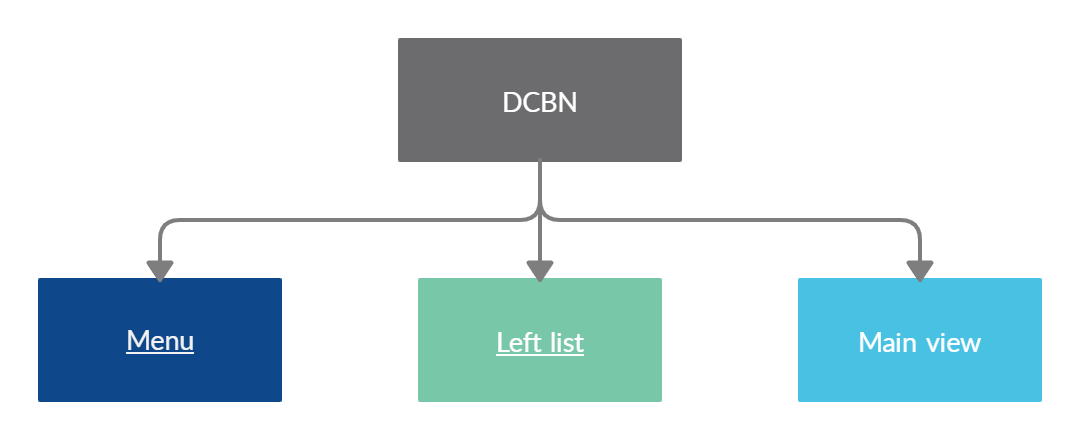
\includegraphics[width=\textwidth,height=\textheight,keepaspectratio]{image/Component_Overview.png}
     \caption{High-Level Ansicht des Diagramms}
\end{figure}
\begin{figure}[ht!]
    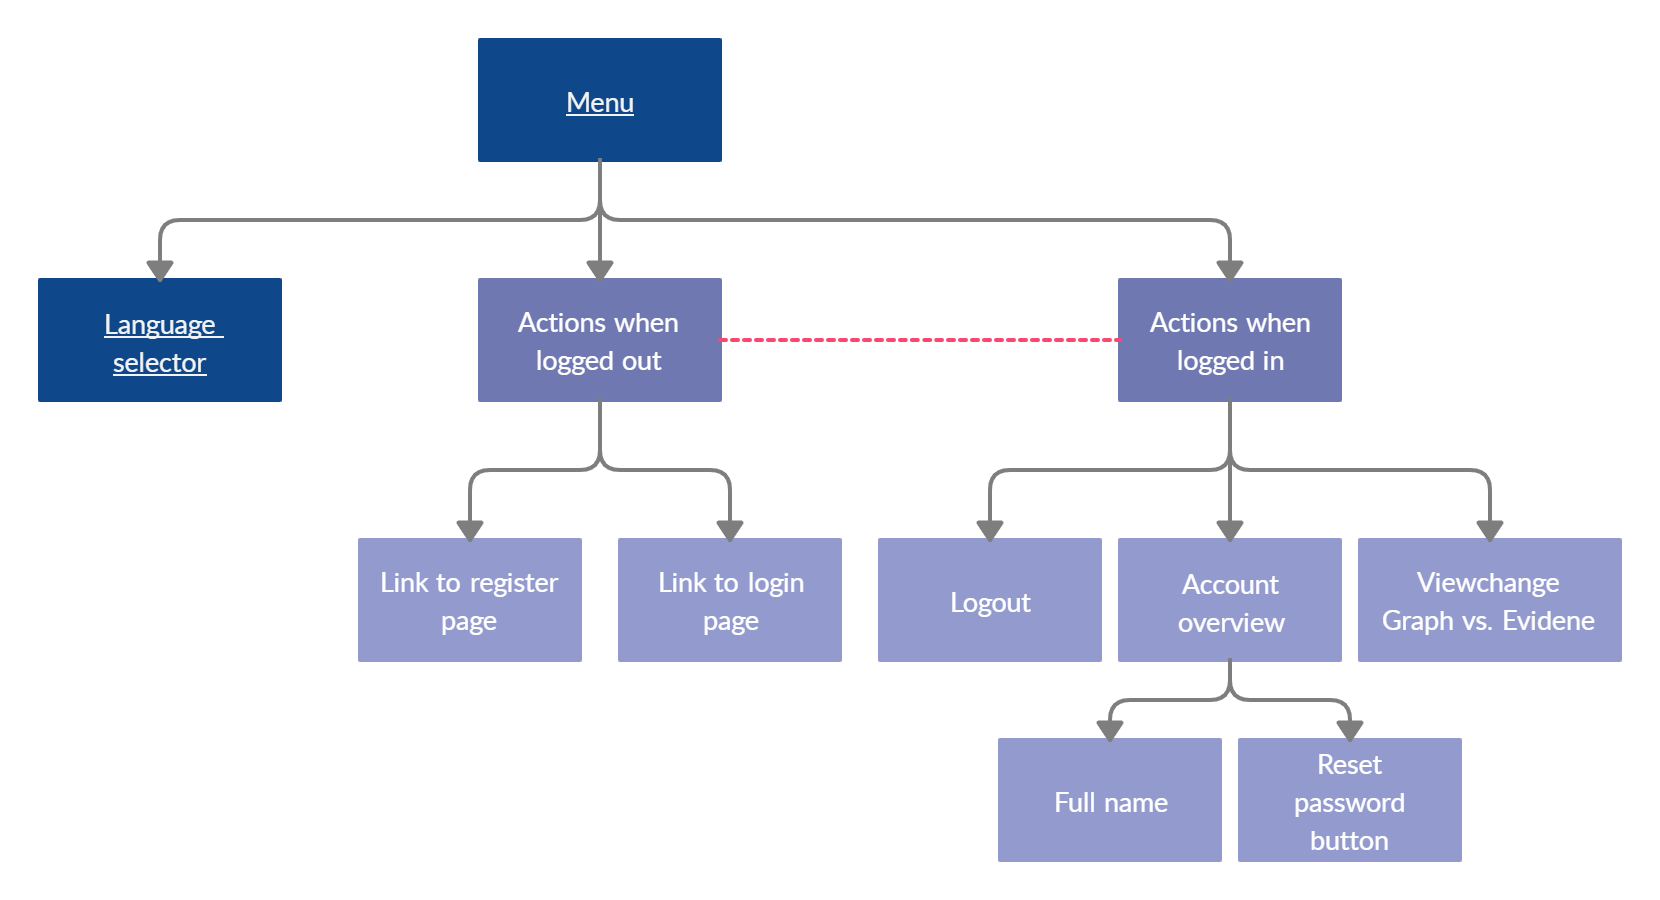
\includegraphics[width=\textwidth,height=\textheight,keepaspectratio]{image/Component_Menu.png}
     \caption{Diagramm des Menüs (Oben im Fenster)}
\end{figure}
\begin{figure}[ht!]
    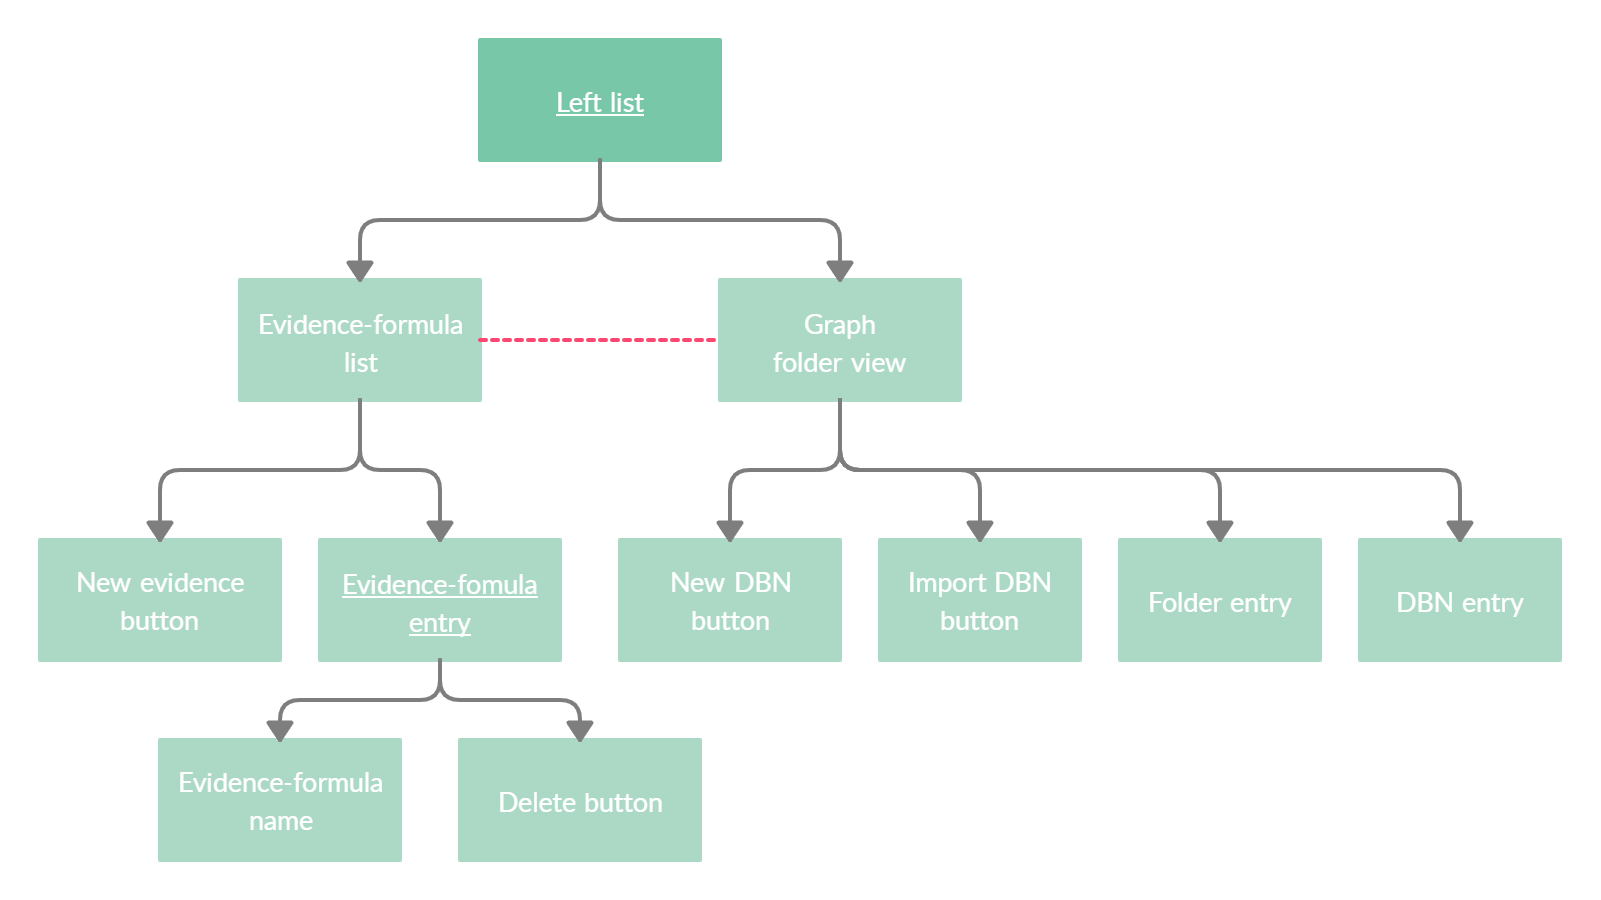
\includegraphics[width=\textwidth,height=\textheight,keepaspectratio]{image/Component_LeftList.png}
     \caption{Diagramm der Liste (Links vom Fenster)}
\end{figure}
\begin{figure}[ht!]
    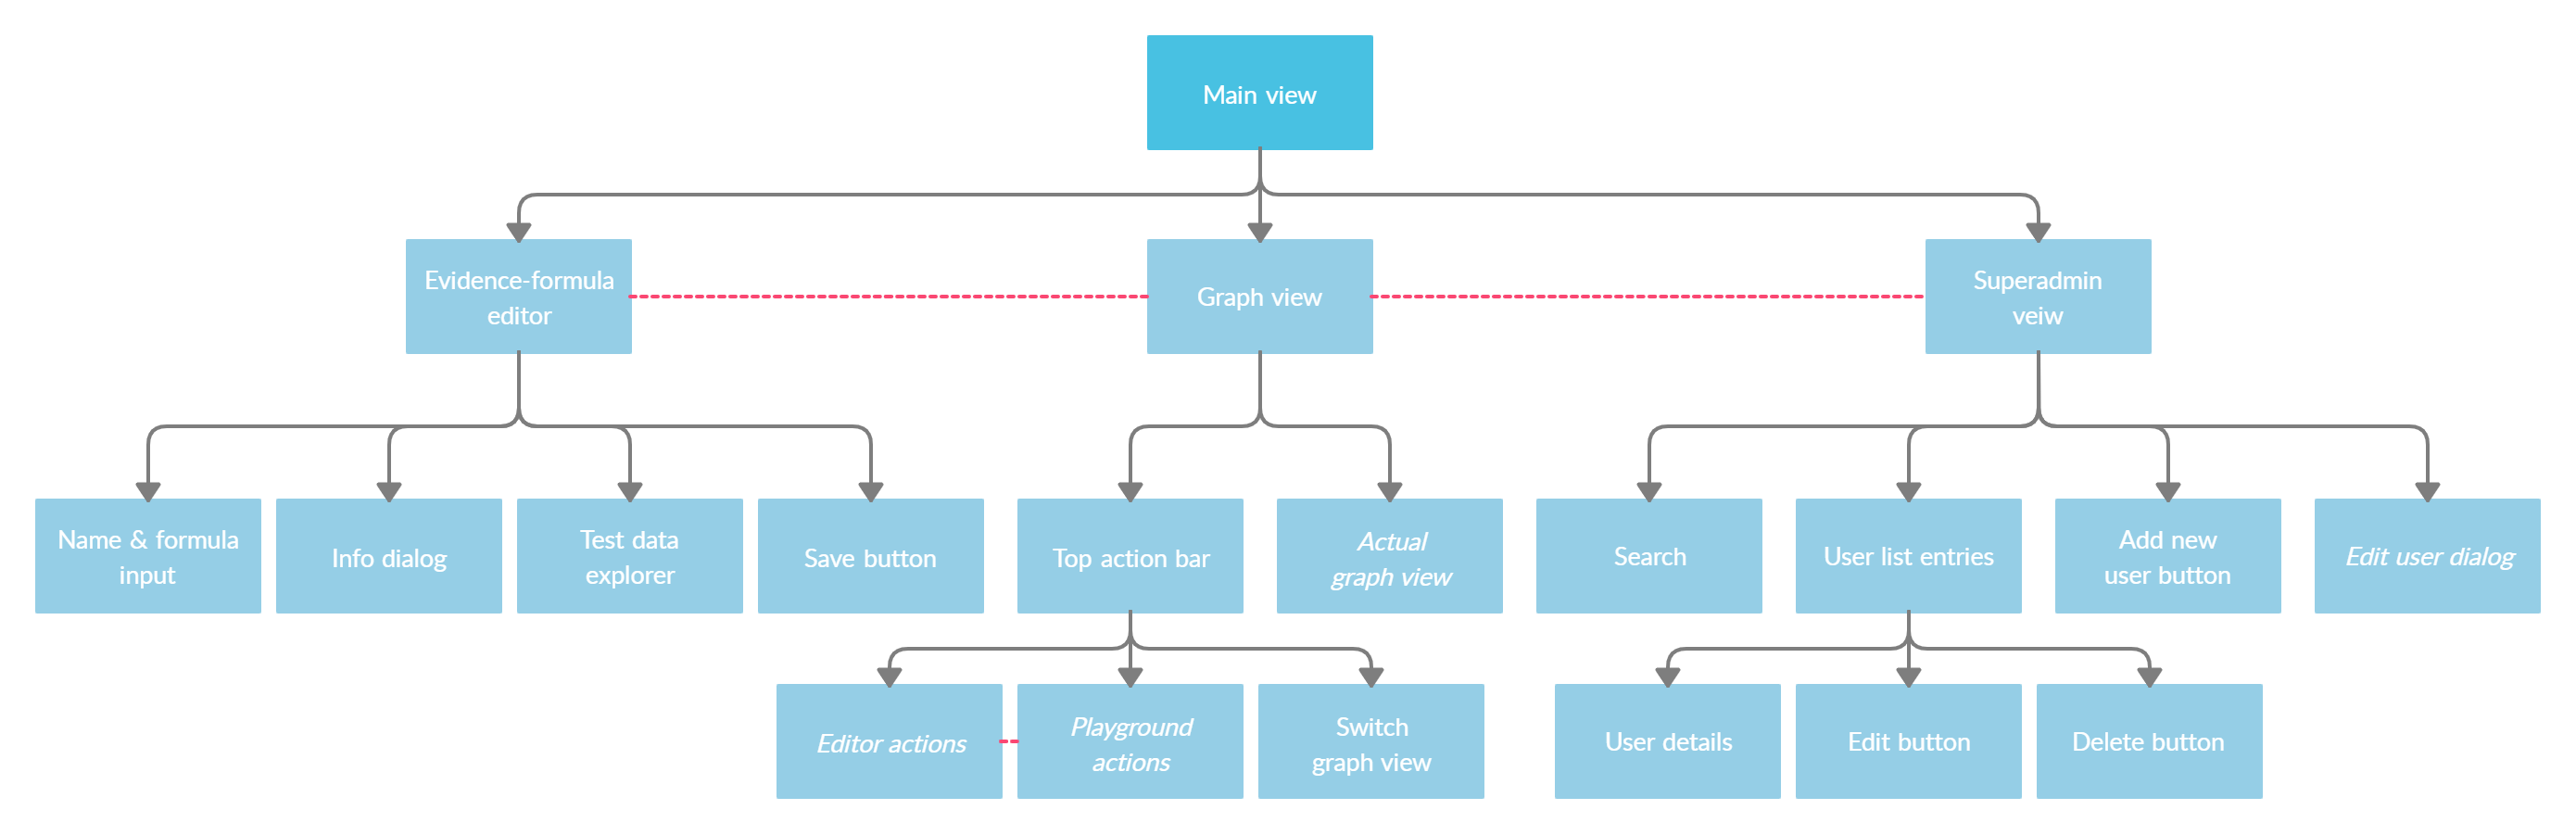
\includegraphics[width=\linewidth]{image/Component_Main.png}
     \caption{Die Main-Komponente des Frontends (Mitte/unten-rechts im Fenster)}
\end{figure}
\newpage
\subsection{Zustandsdiagramm der Benutzerverwaltung}
\begin{figure}[ht!]
    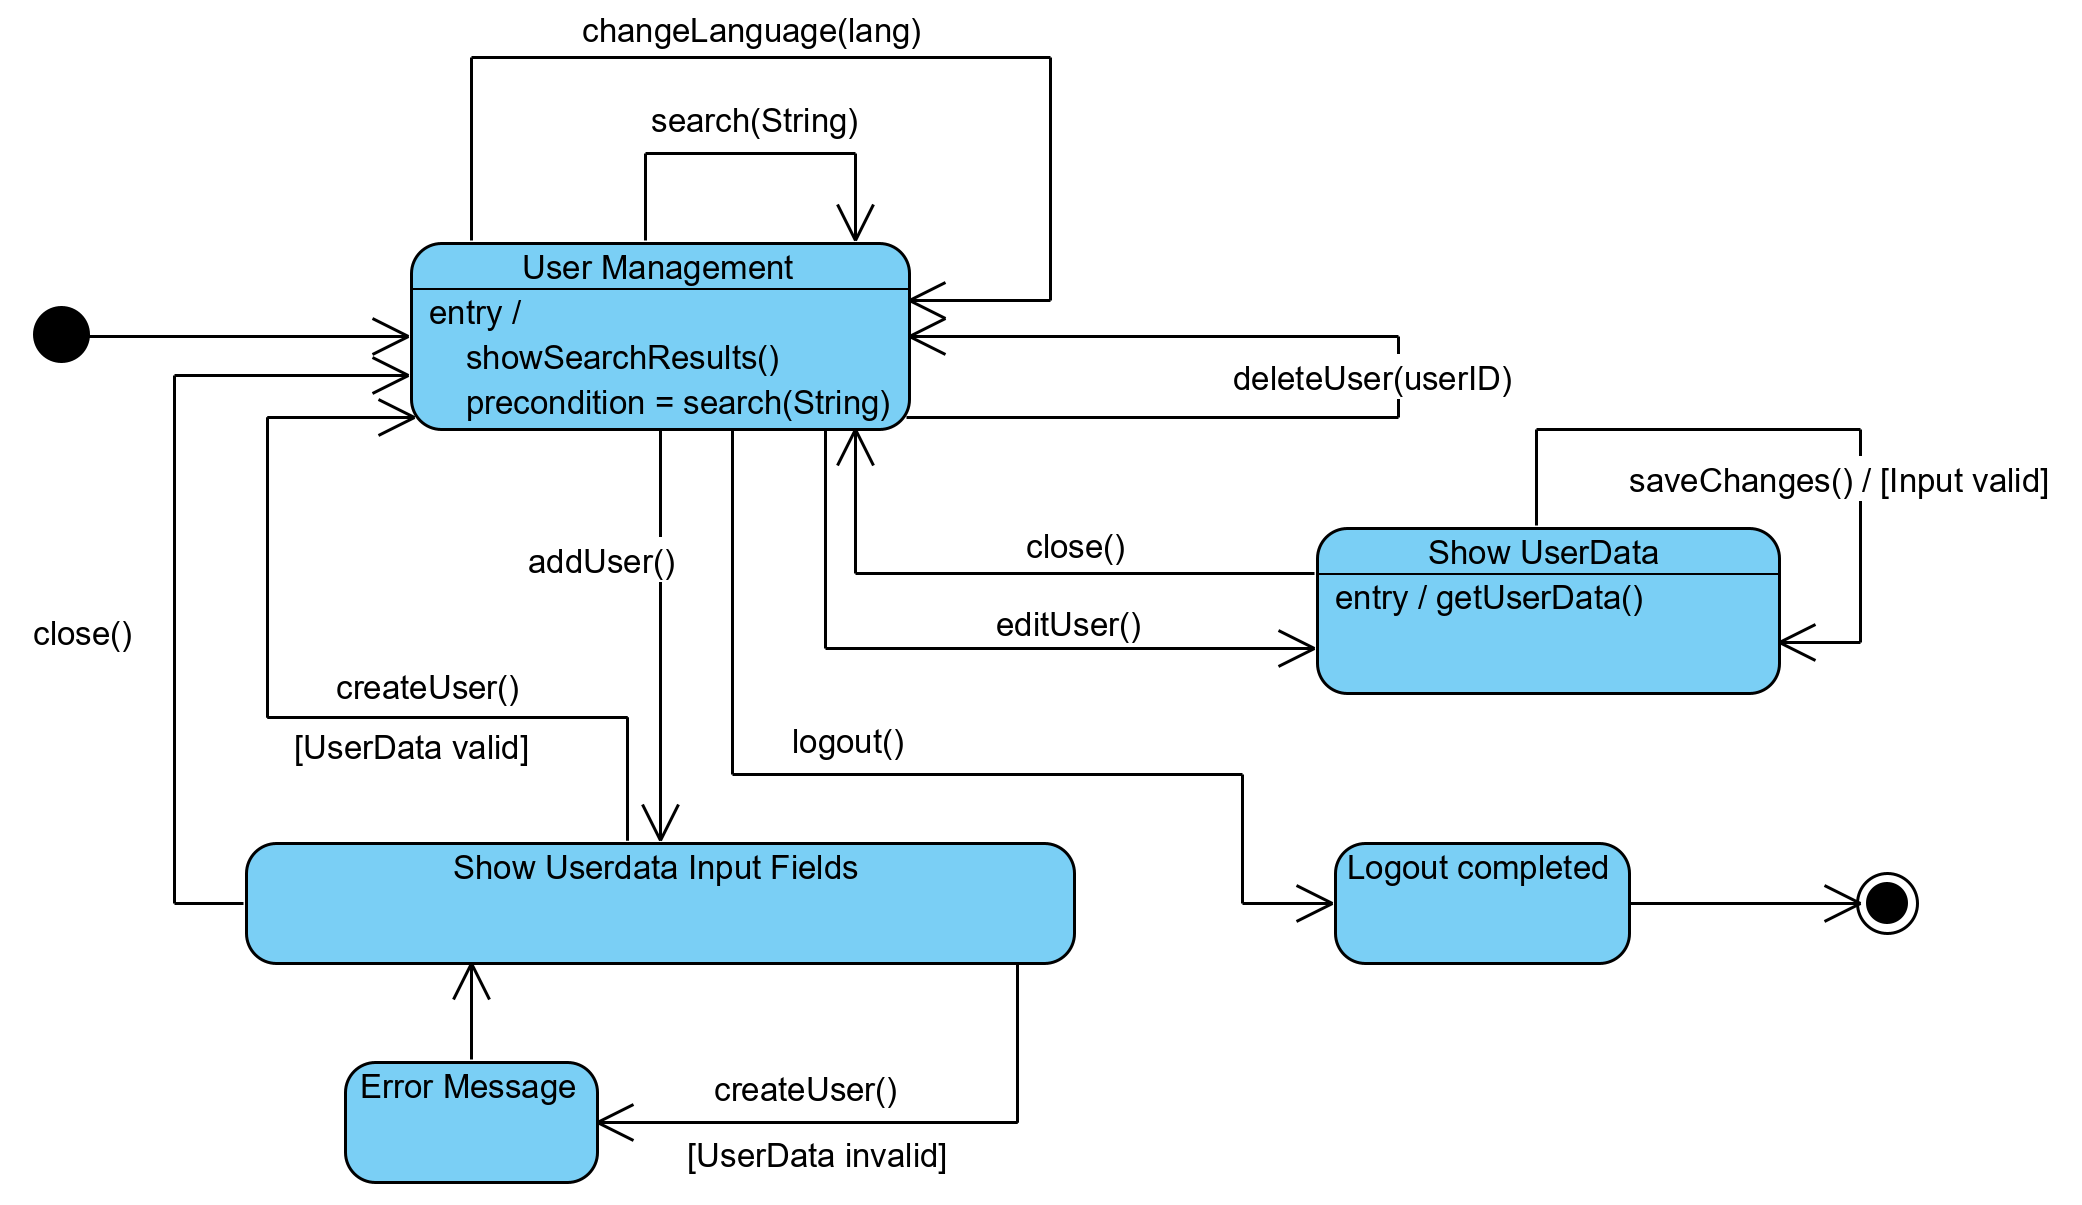
\includegraphics[width=\linewidth]{image/Benutzerverwaltung.png}
    \caption{Das Zustandsdiagramm der Benutzerverwaltung}
\end{figure}
\newpage
\subsection{Zustandsdiagramm der Login-Seite}
\begin{figure}[ht!]
    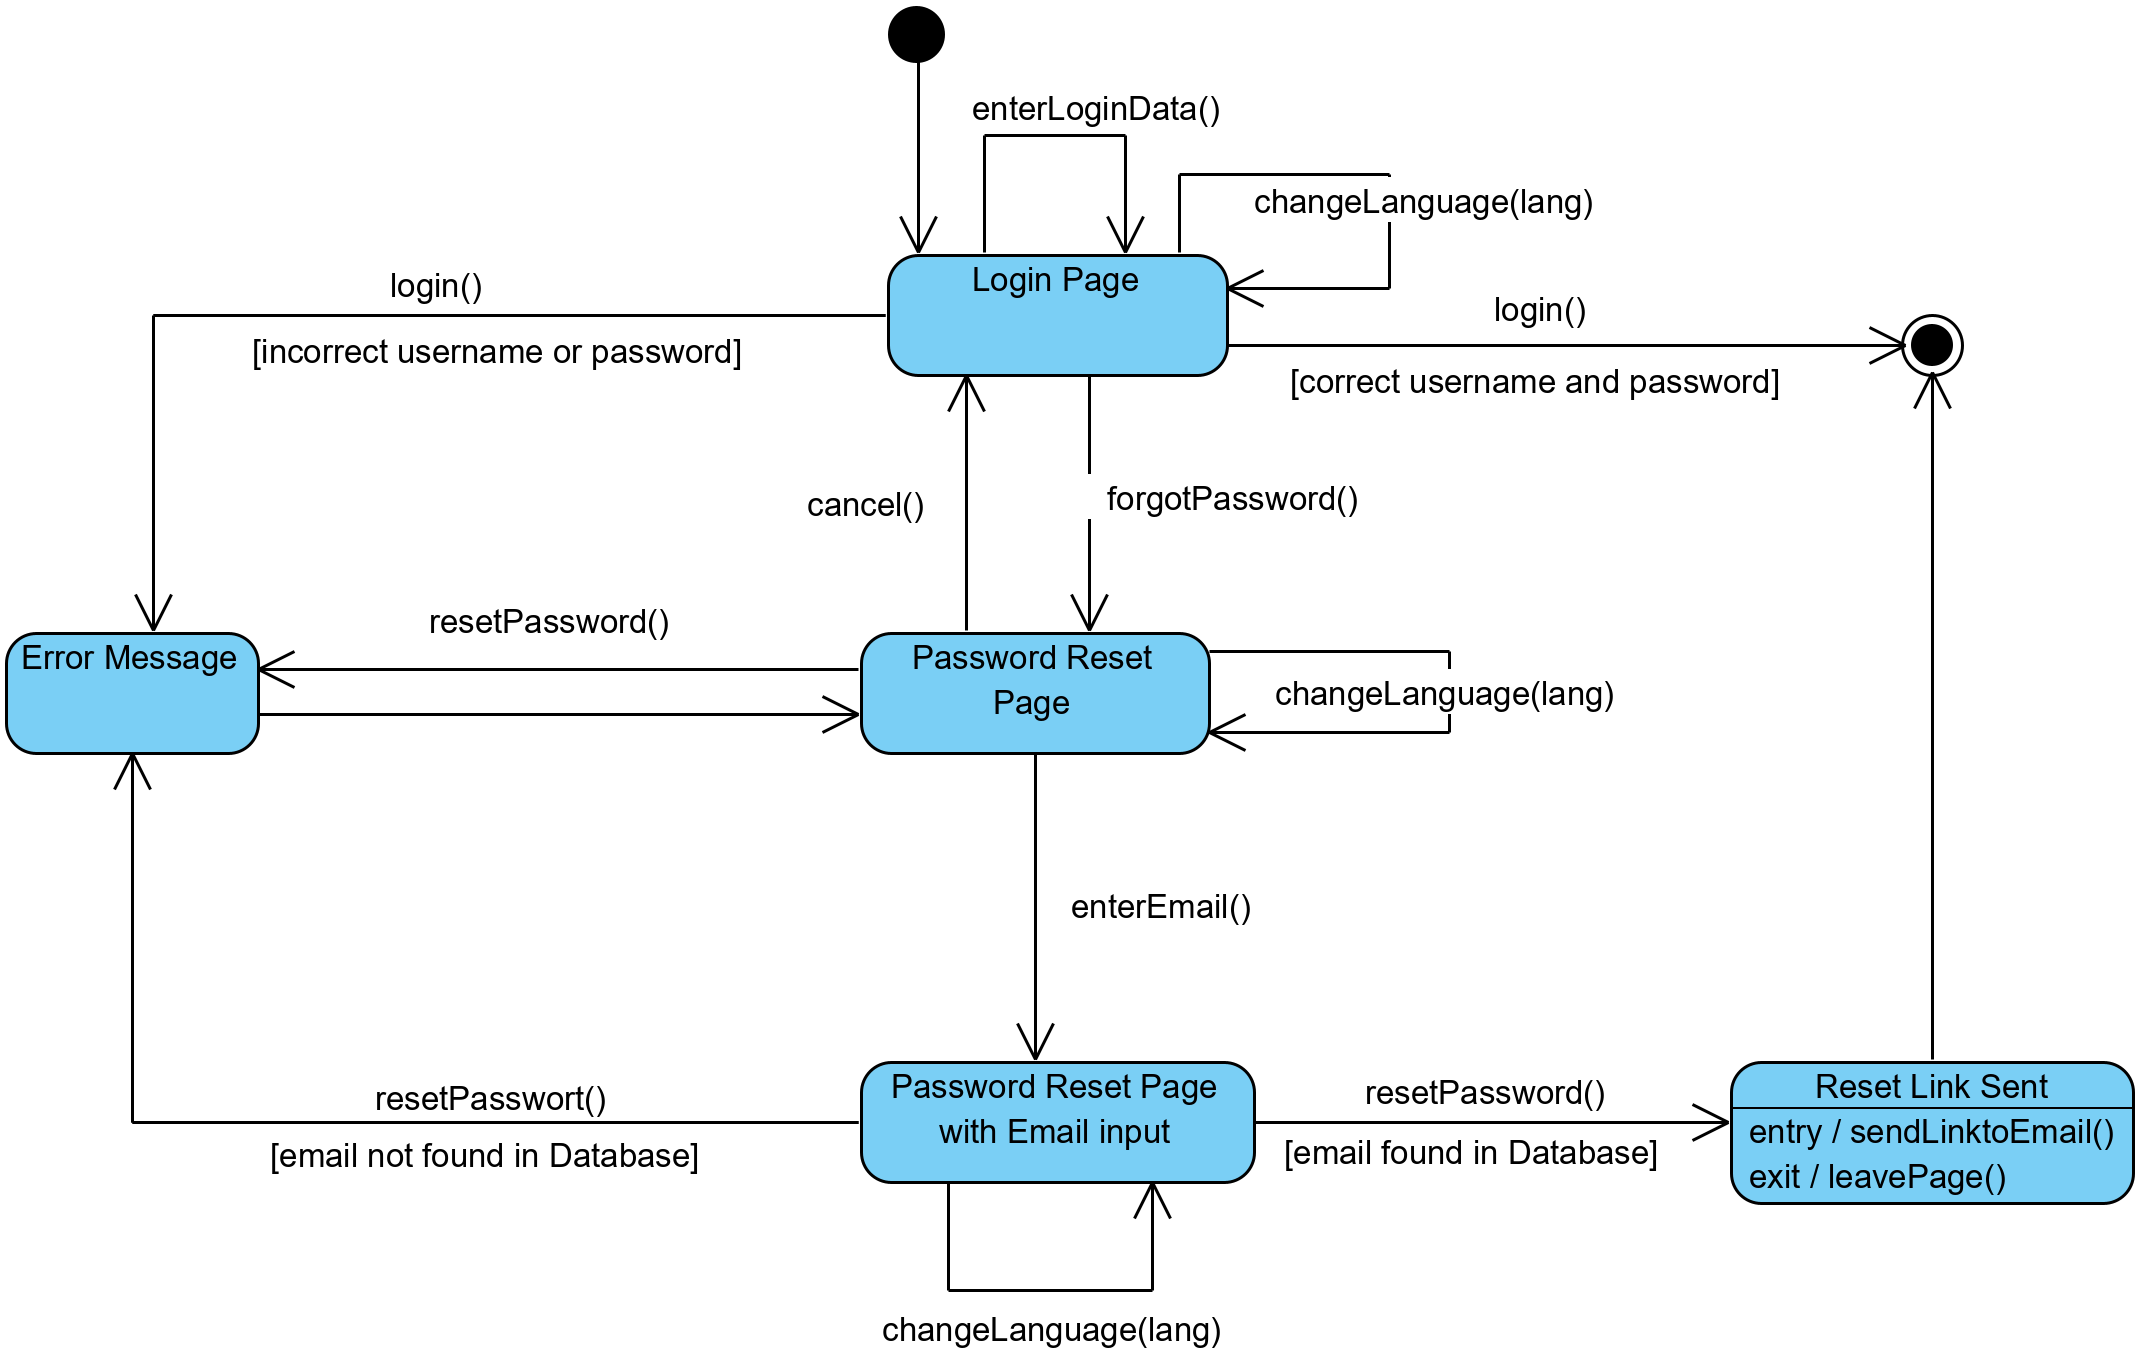
\includegraphics[width=\linewidth]{image/Anmeldeseite.png}
    \caption{Das Zustandsdiagramm der Anmeldeseite}
\end{figure}

\newpage
\subsection{Aktivitätsdiagramm zur Erstellung einer Evidenz}

\begin{figure}[ht!]
    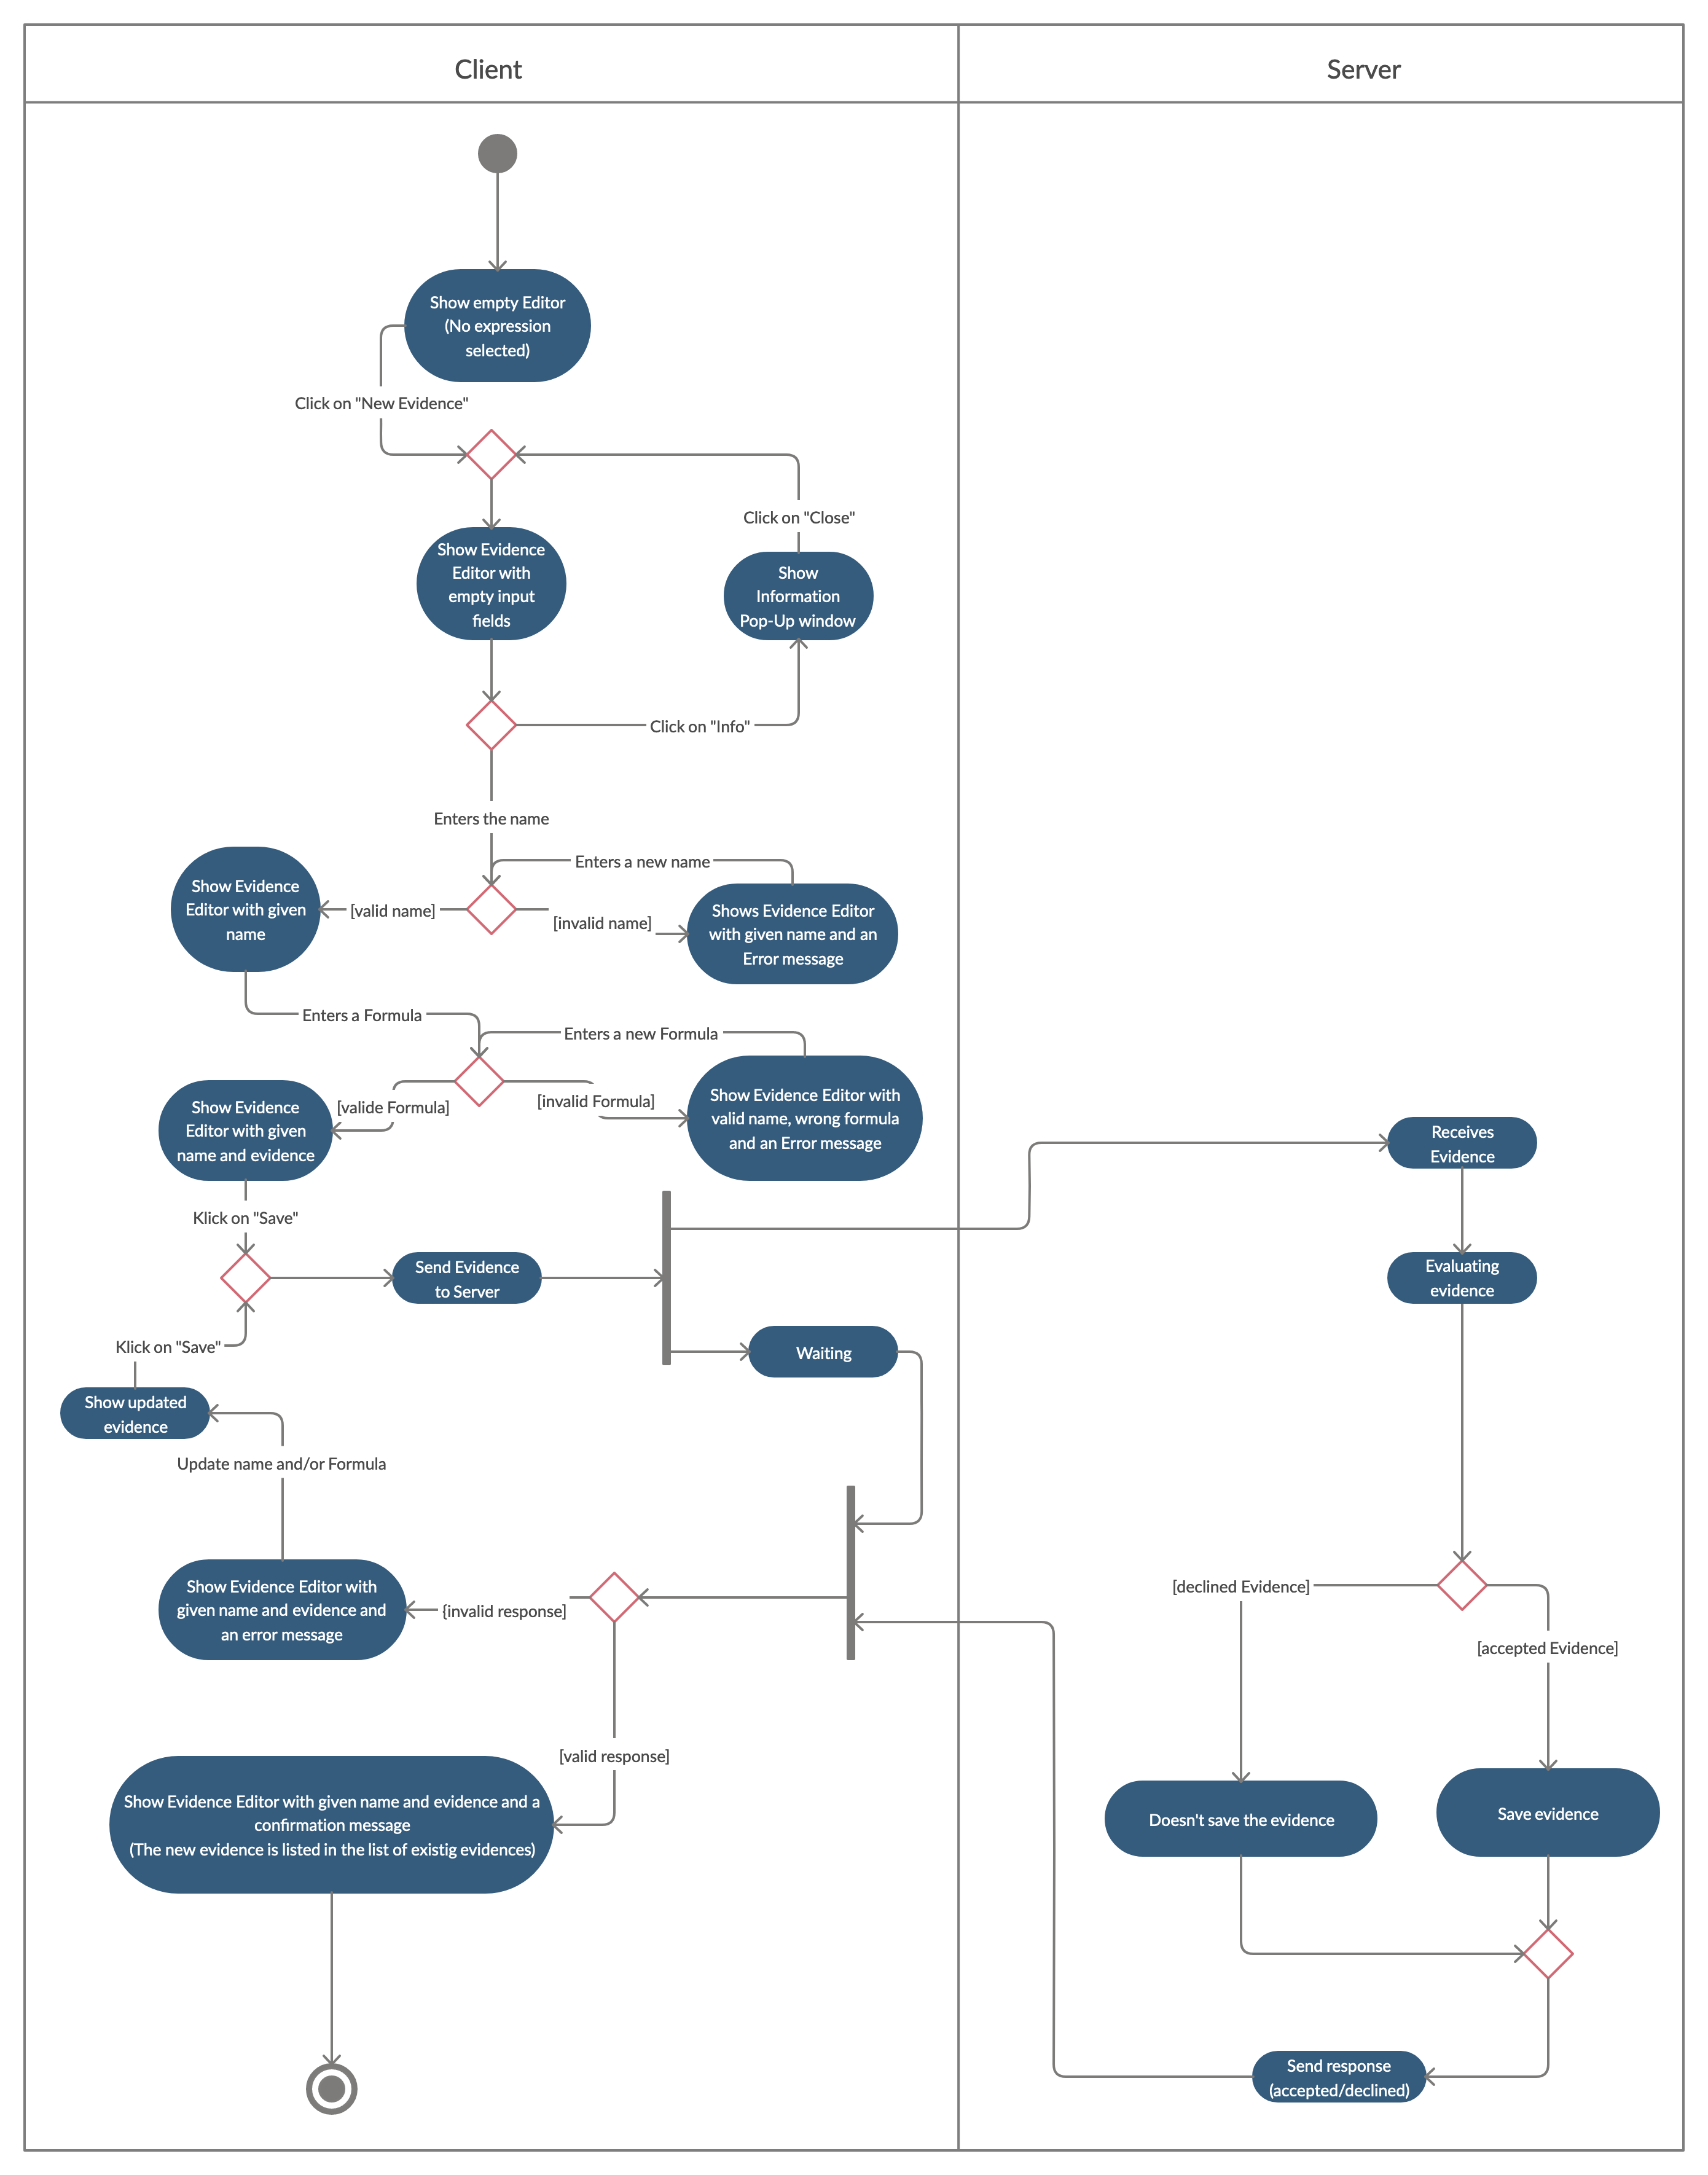
\includegraphics[width=\textwidth,height=\textheight,keepaspectratio]{image/Activity_EvidenceFormular.png}
    \caption{Dieses Aktivitätsdiagramm beschreibt die Erstellung einer neuen Evidenz-Formel}
\end{figure}

\newpage
\subsection{Aktivitätsdiagramm zur Benutzung des Graph-Editors}
\begin{figure}[ht!]
    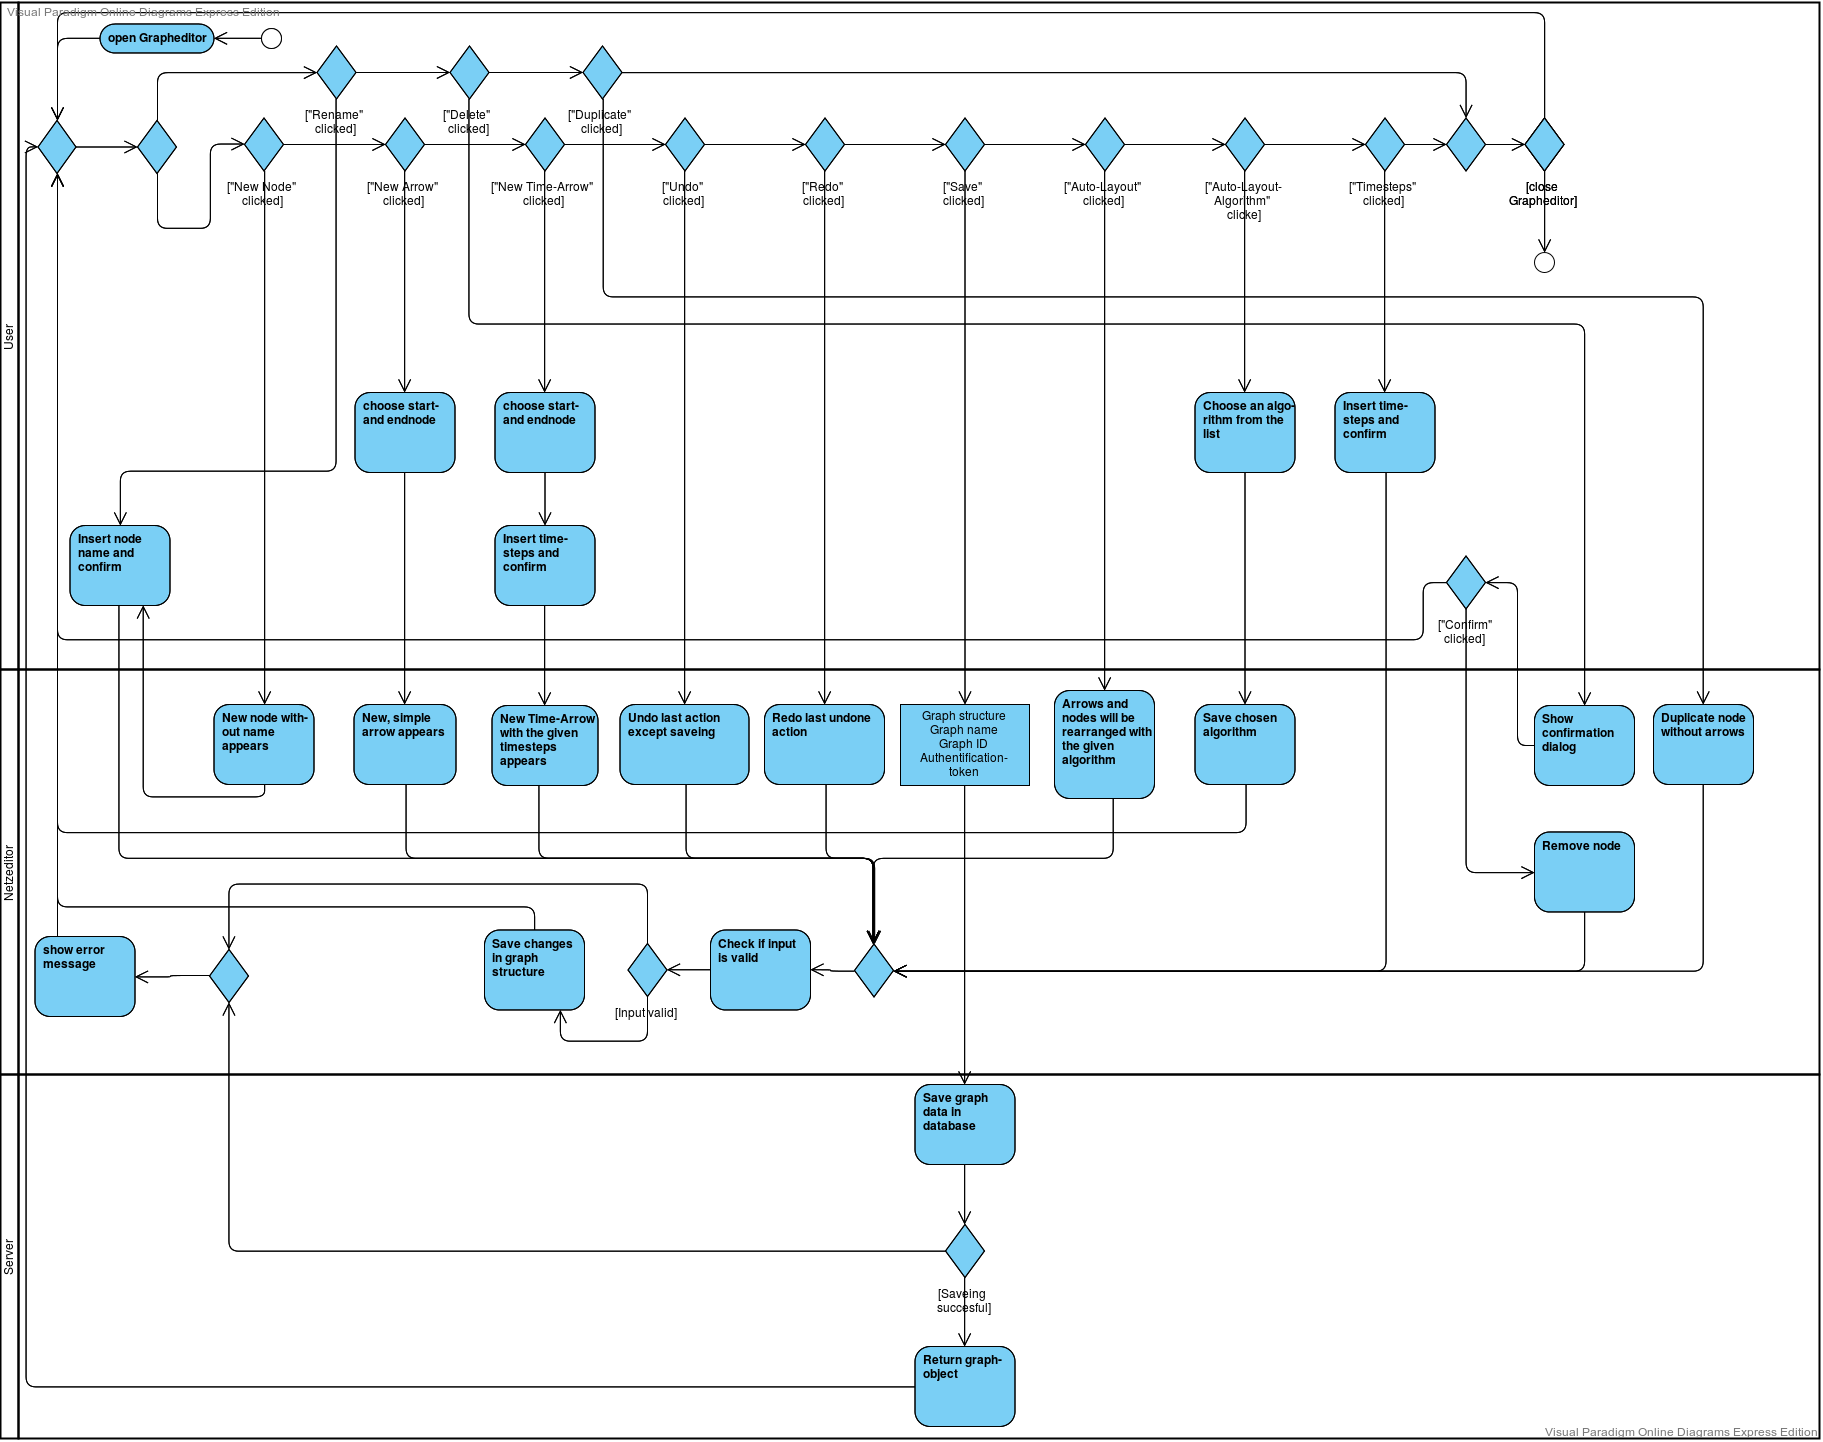
\includegraphics[width=\textwidth,height=\textheight,keepaspectratio]{image/Activity_Grapheditor.png}
    \caption{Dieses Aktivitätsdiagramm beschreibt die Funktionen des Graph-Editors }
\end{figure}
\newpage

\section{REST-Schnittstelle}

\subsection{Login}
\begin{figure}[ht!]
    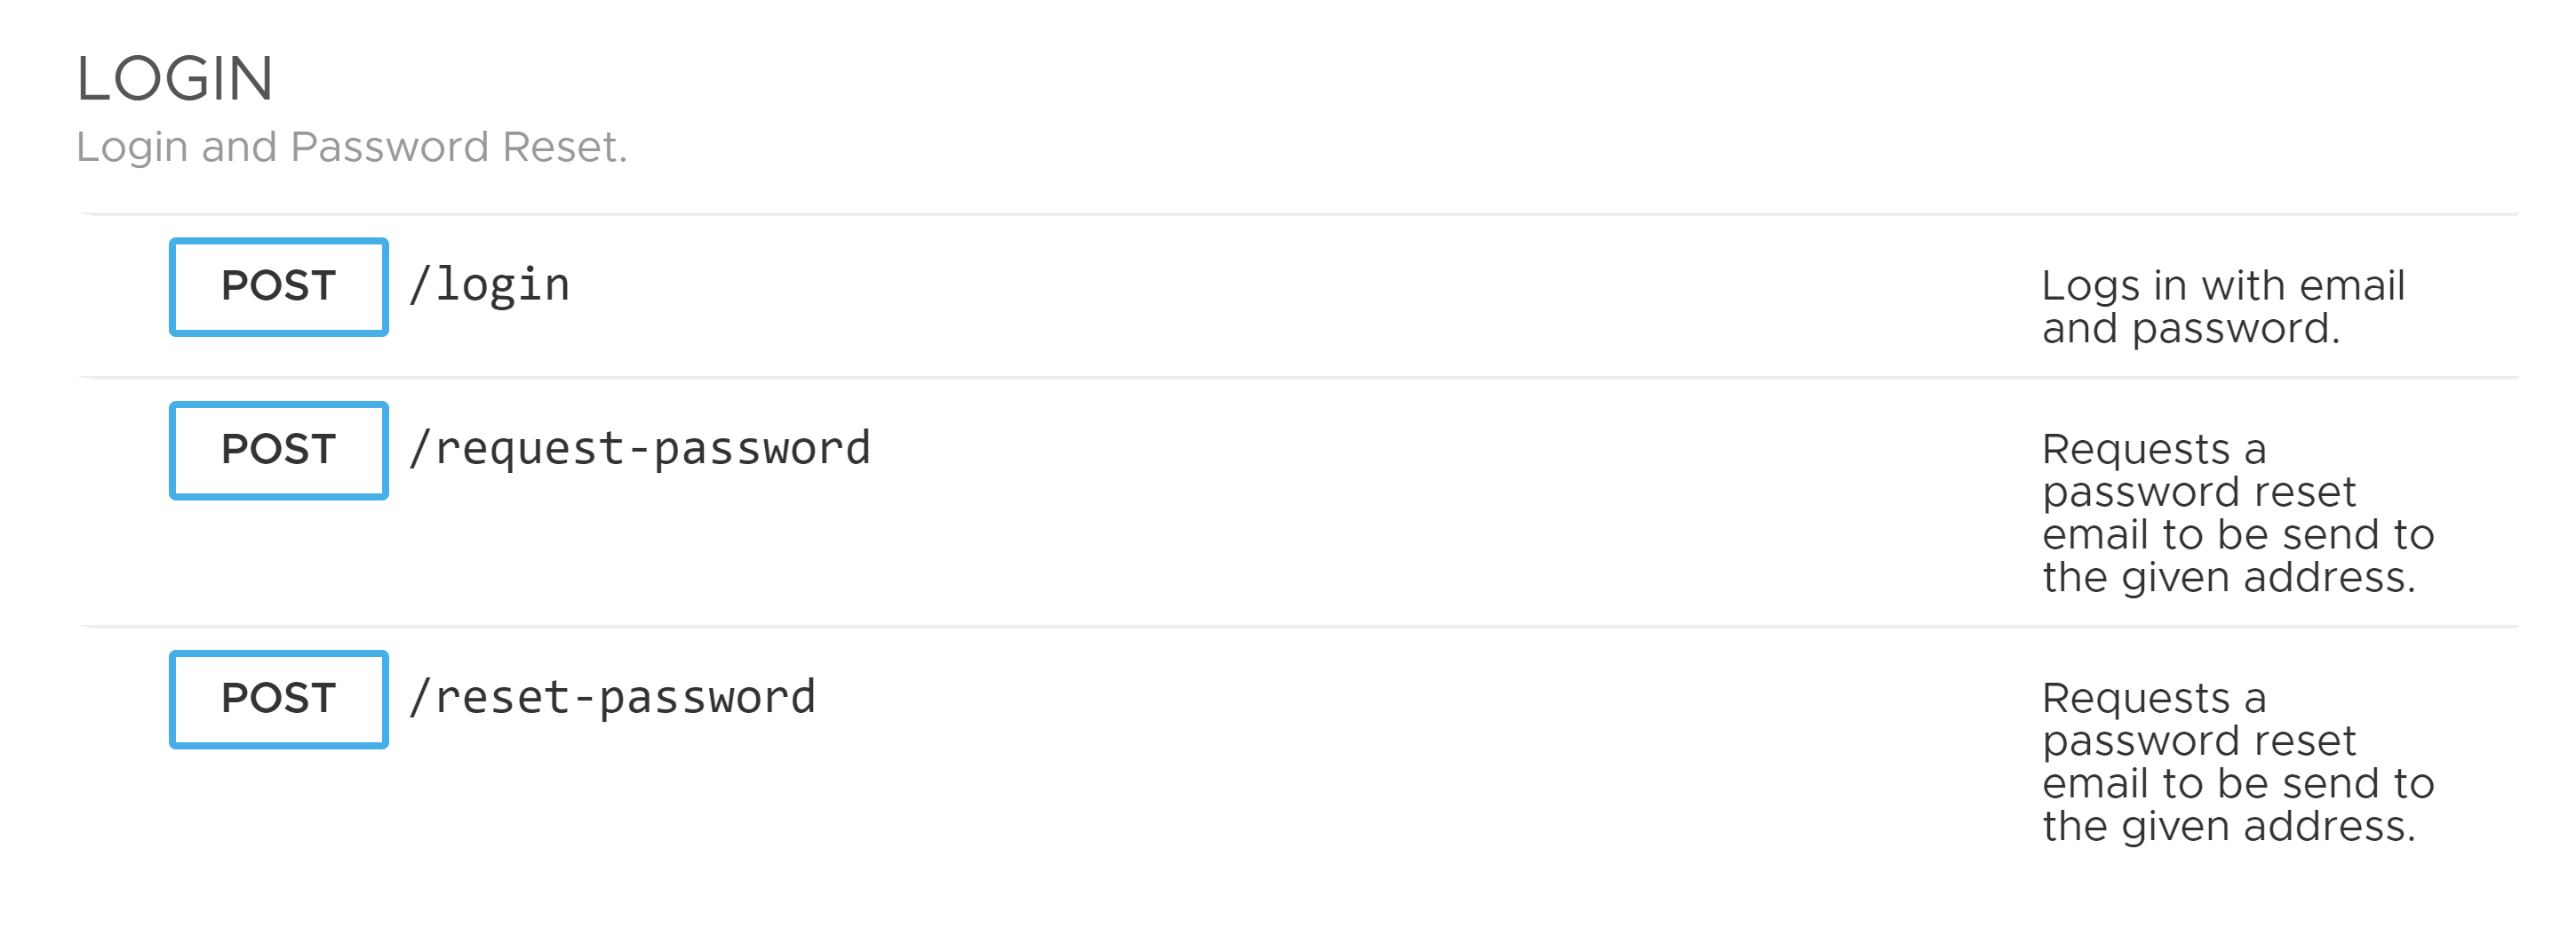
\includegraphics[width=\linewidth]{image/REST_Login.png}
    \caption{REST Schnittstelle für Login}
\end{figure}


\subsection{Users}
\begin{figure}[ht!]
    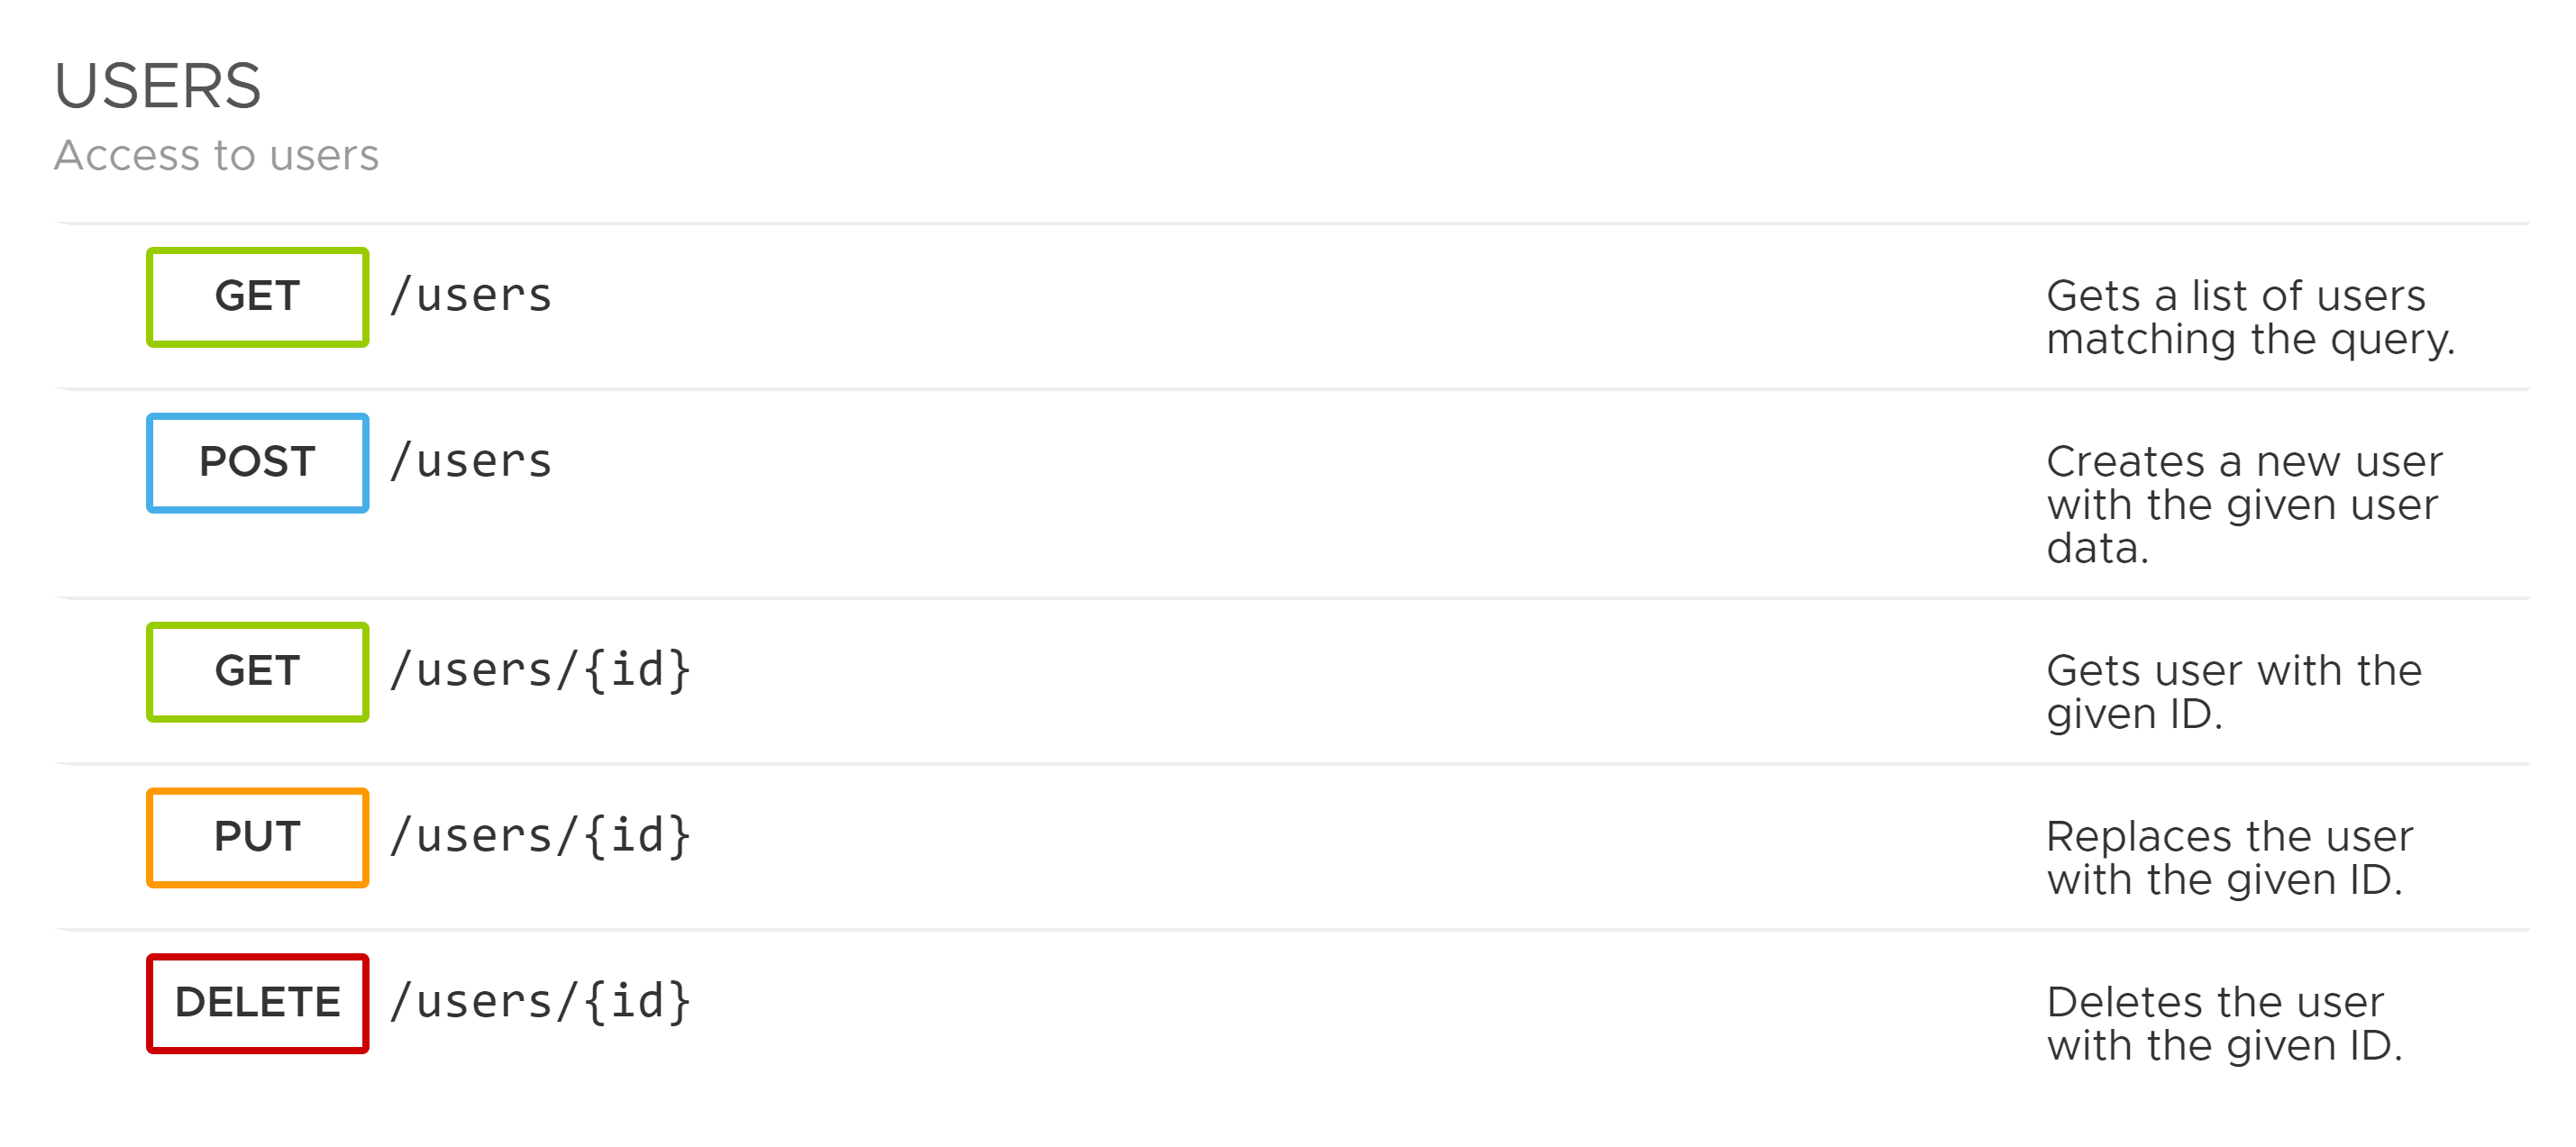
\includegraphics[width=\linewidth]{image/REST_Users.png}
    \caption{REST Schnittstelle für Nutzersystem}
\end{figure}
\newpage
\subsection{Graphs}
\begin{figure}[ht!]
    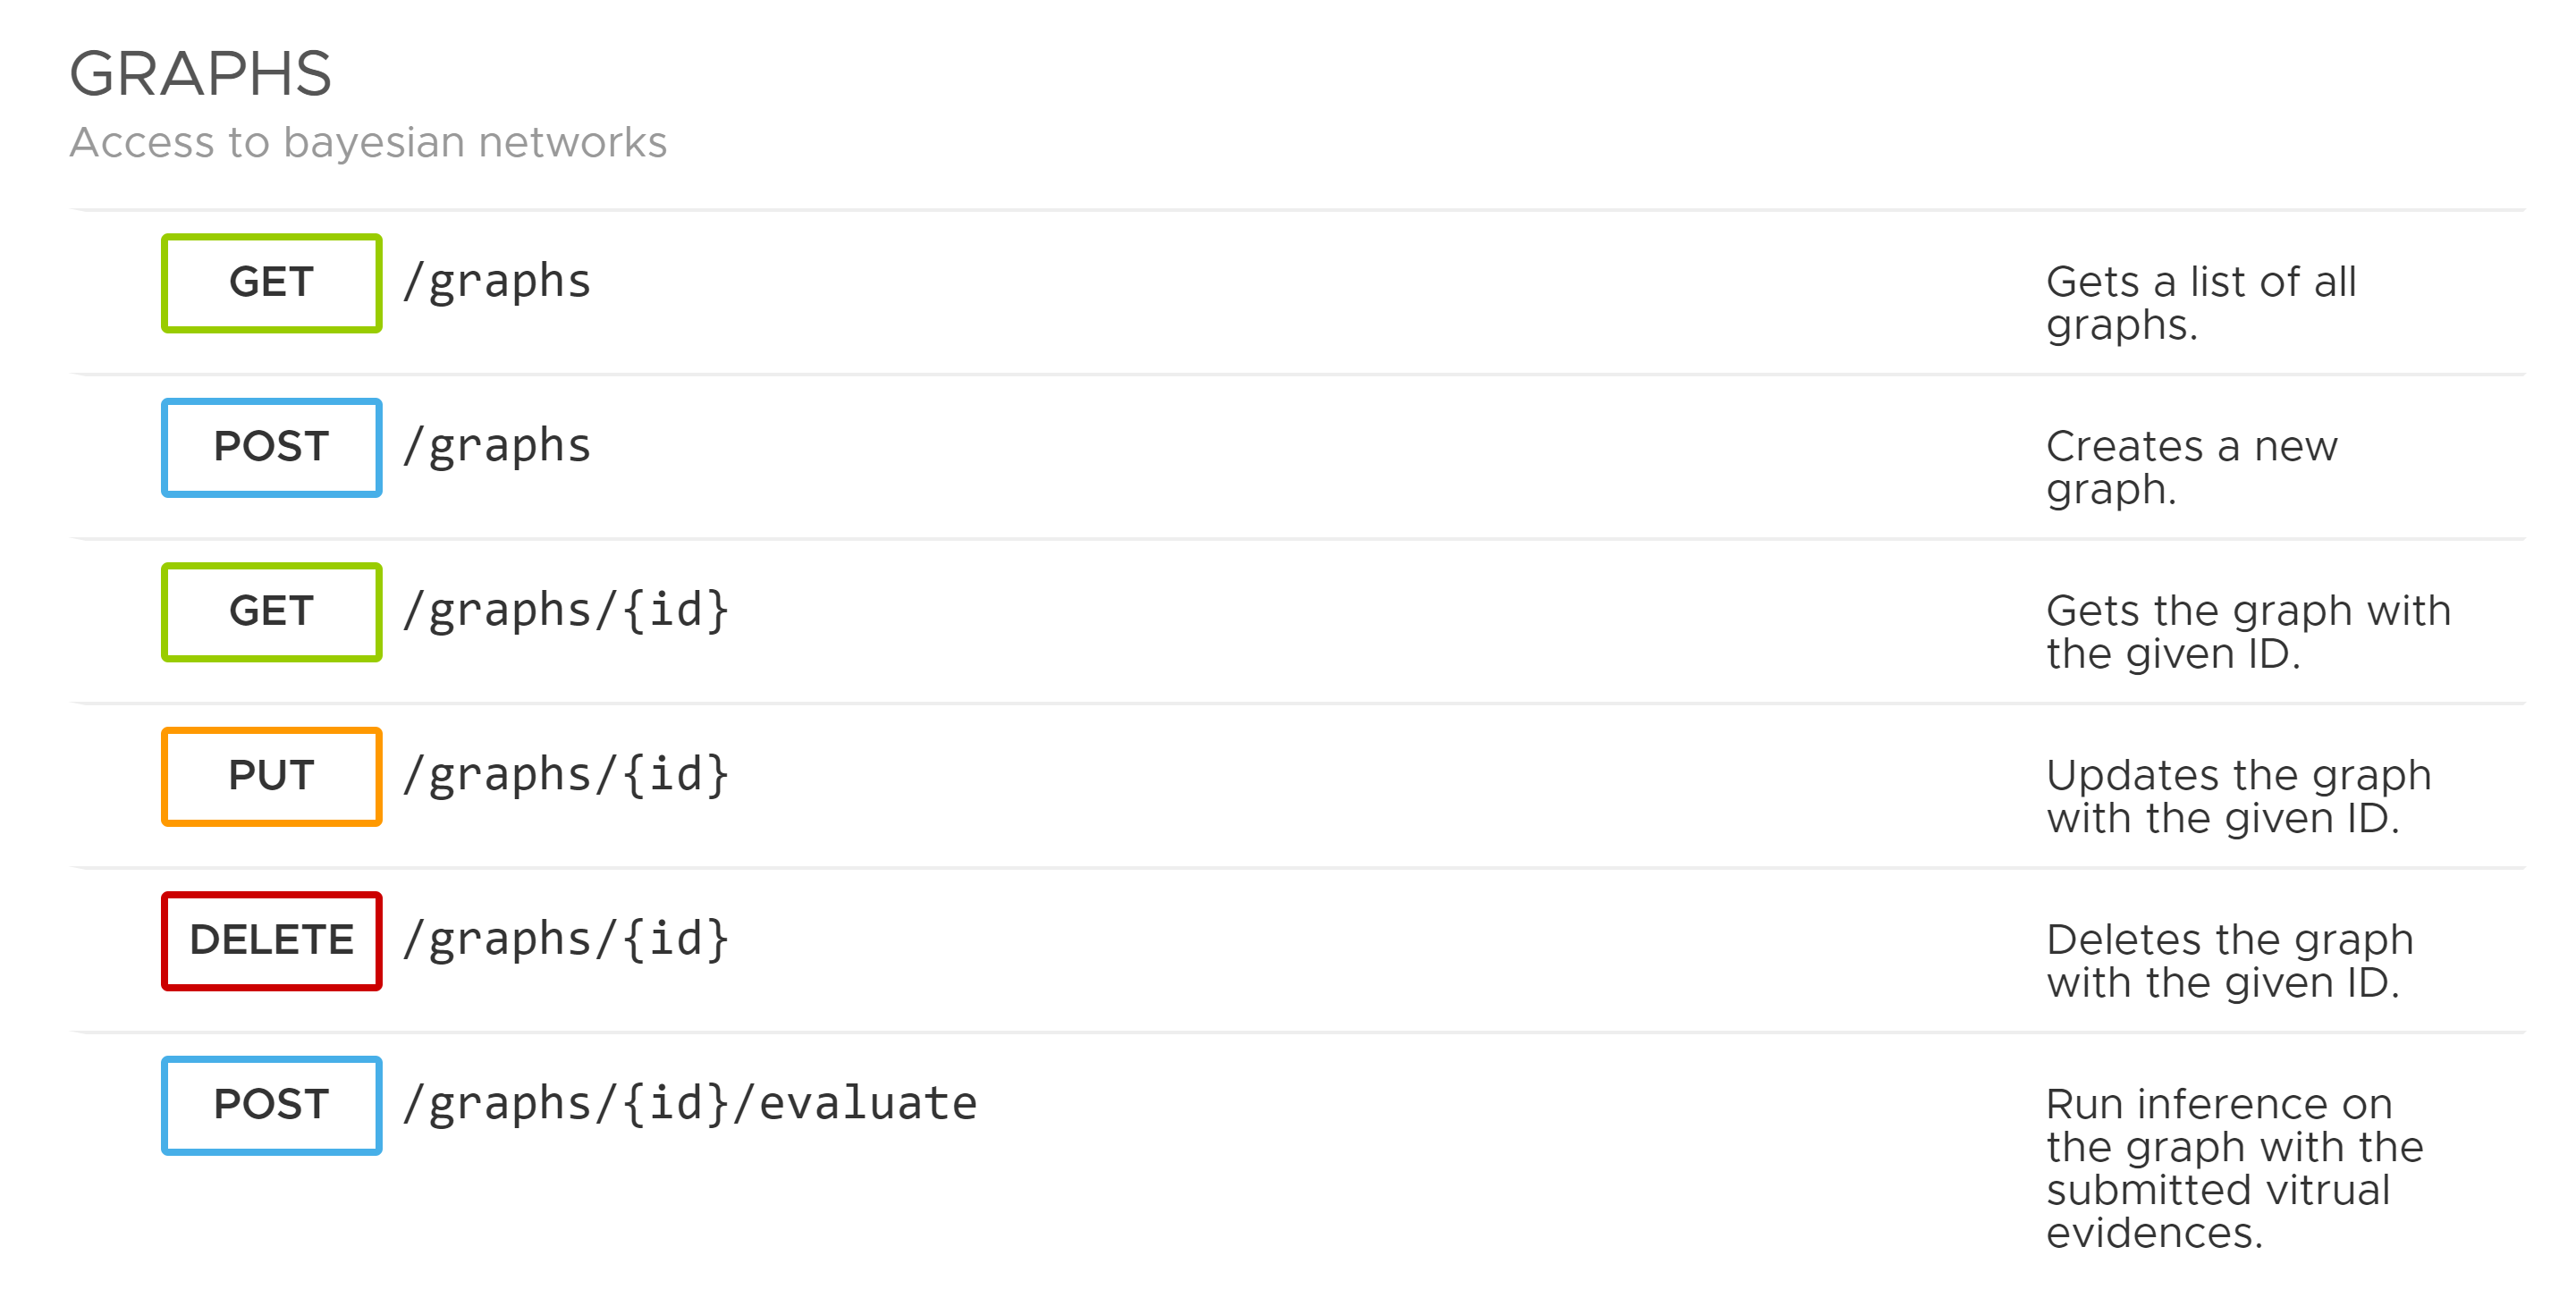
\includegraphics[width=\linewidth]{image/REST_Graphs.png}
    \caption{REST Schnittstelle für Netze}
\end{figure}
\subsection{Evidenz-Formeln}
\begin{figure}[ht!]
    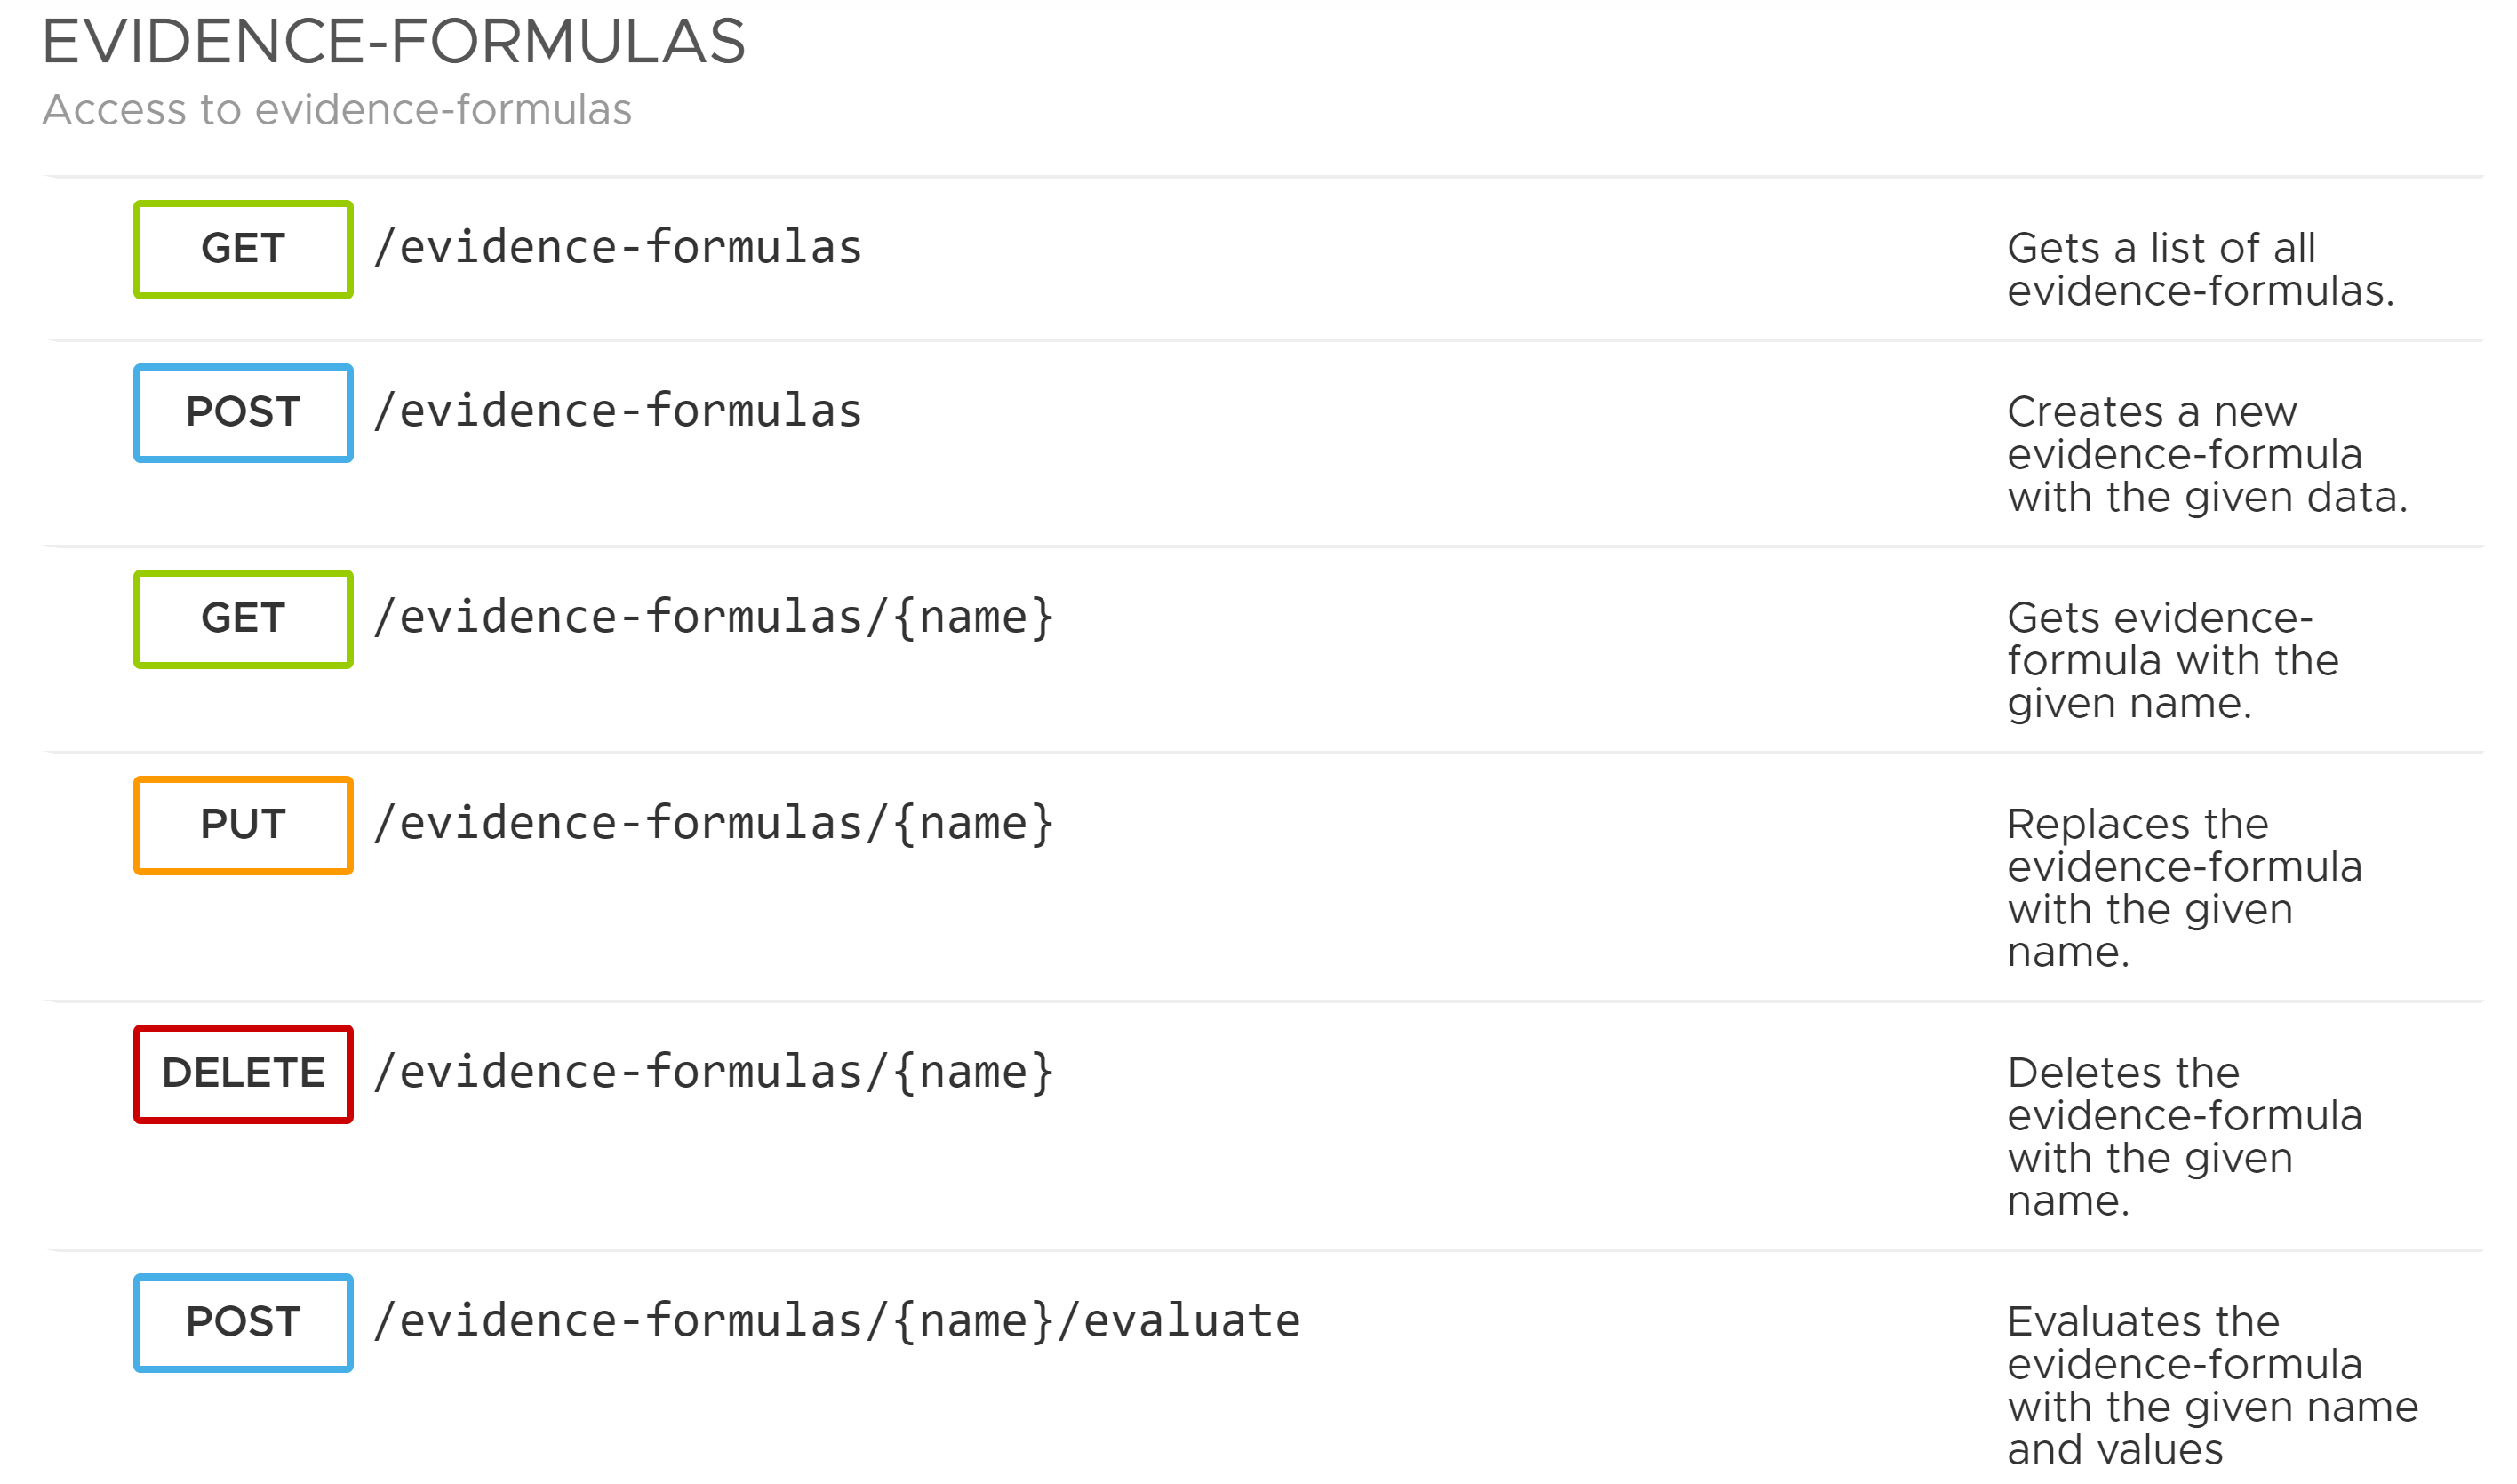
\includegraphics[width=\linewidth]{image/REST_Evid.png}
    \caption{REST Schnittstelle für Evidenzen}
\end{figure}

\section{Backend}
\subsection{REST}
\begin{figure}[ht!]
    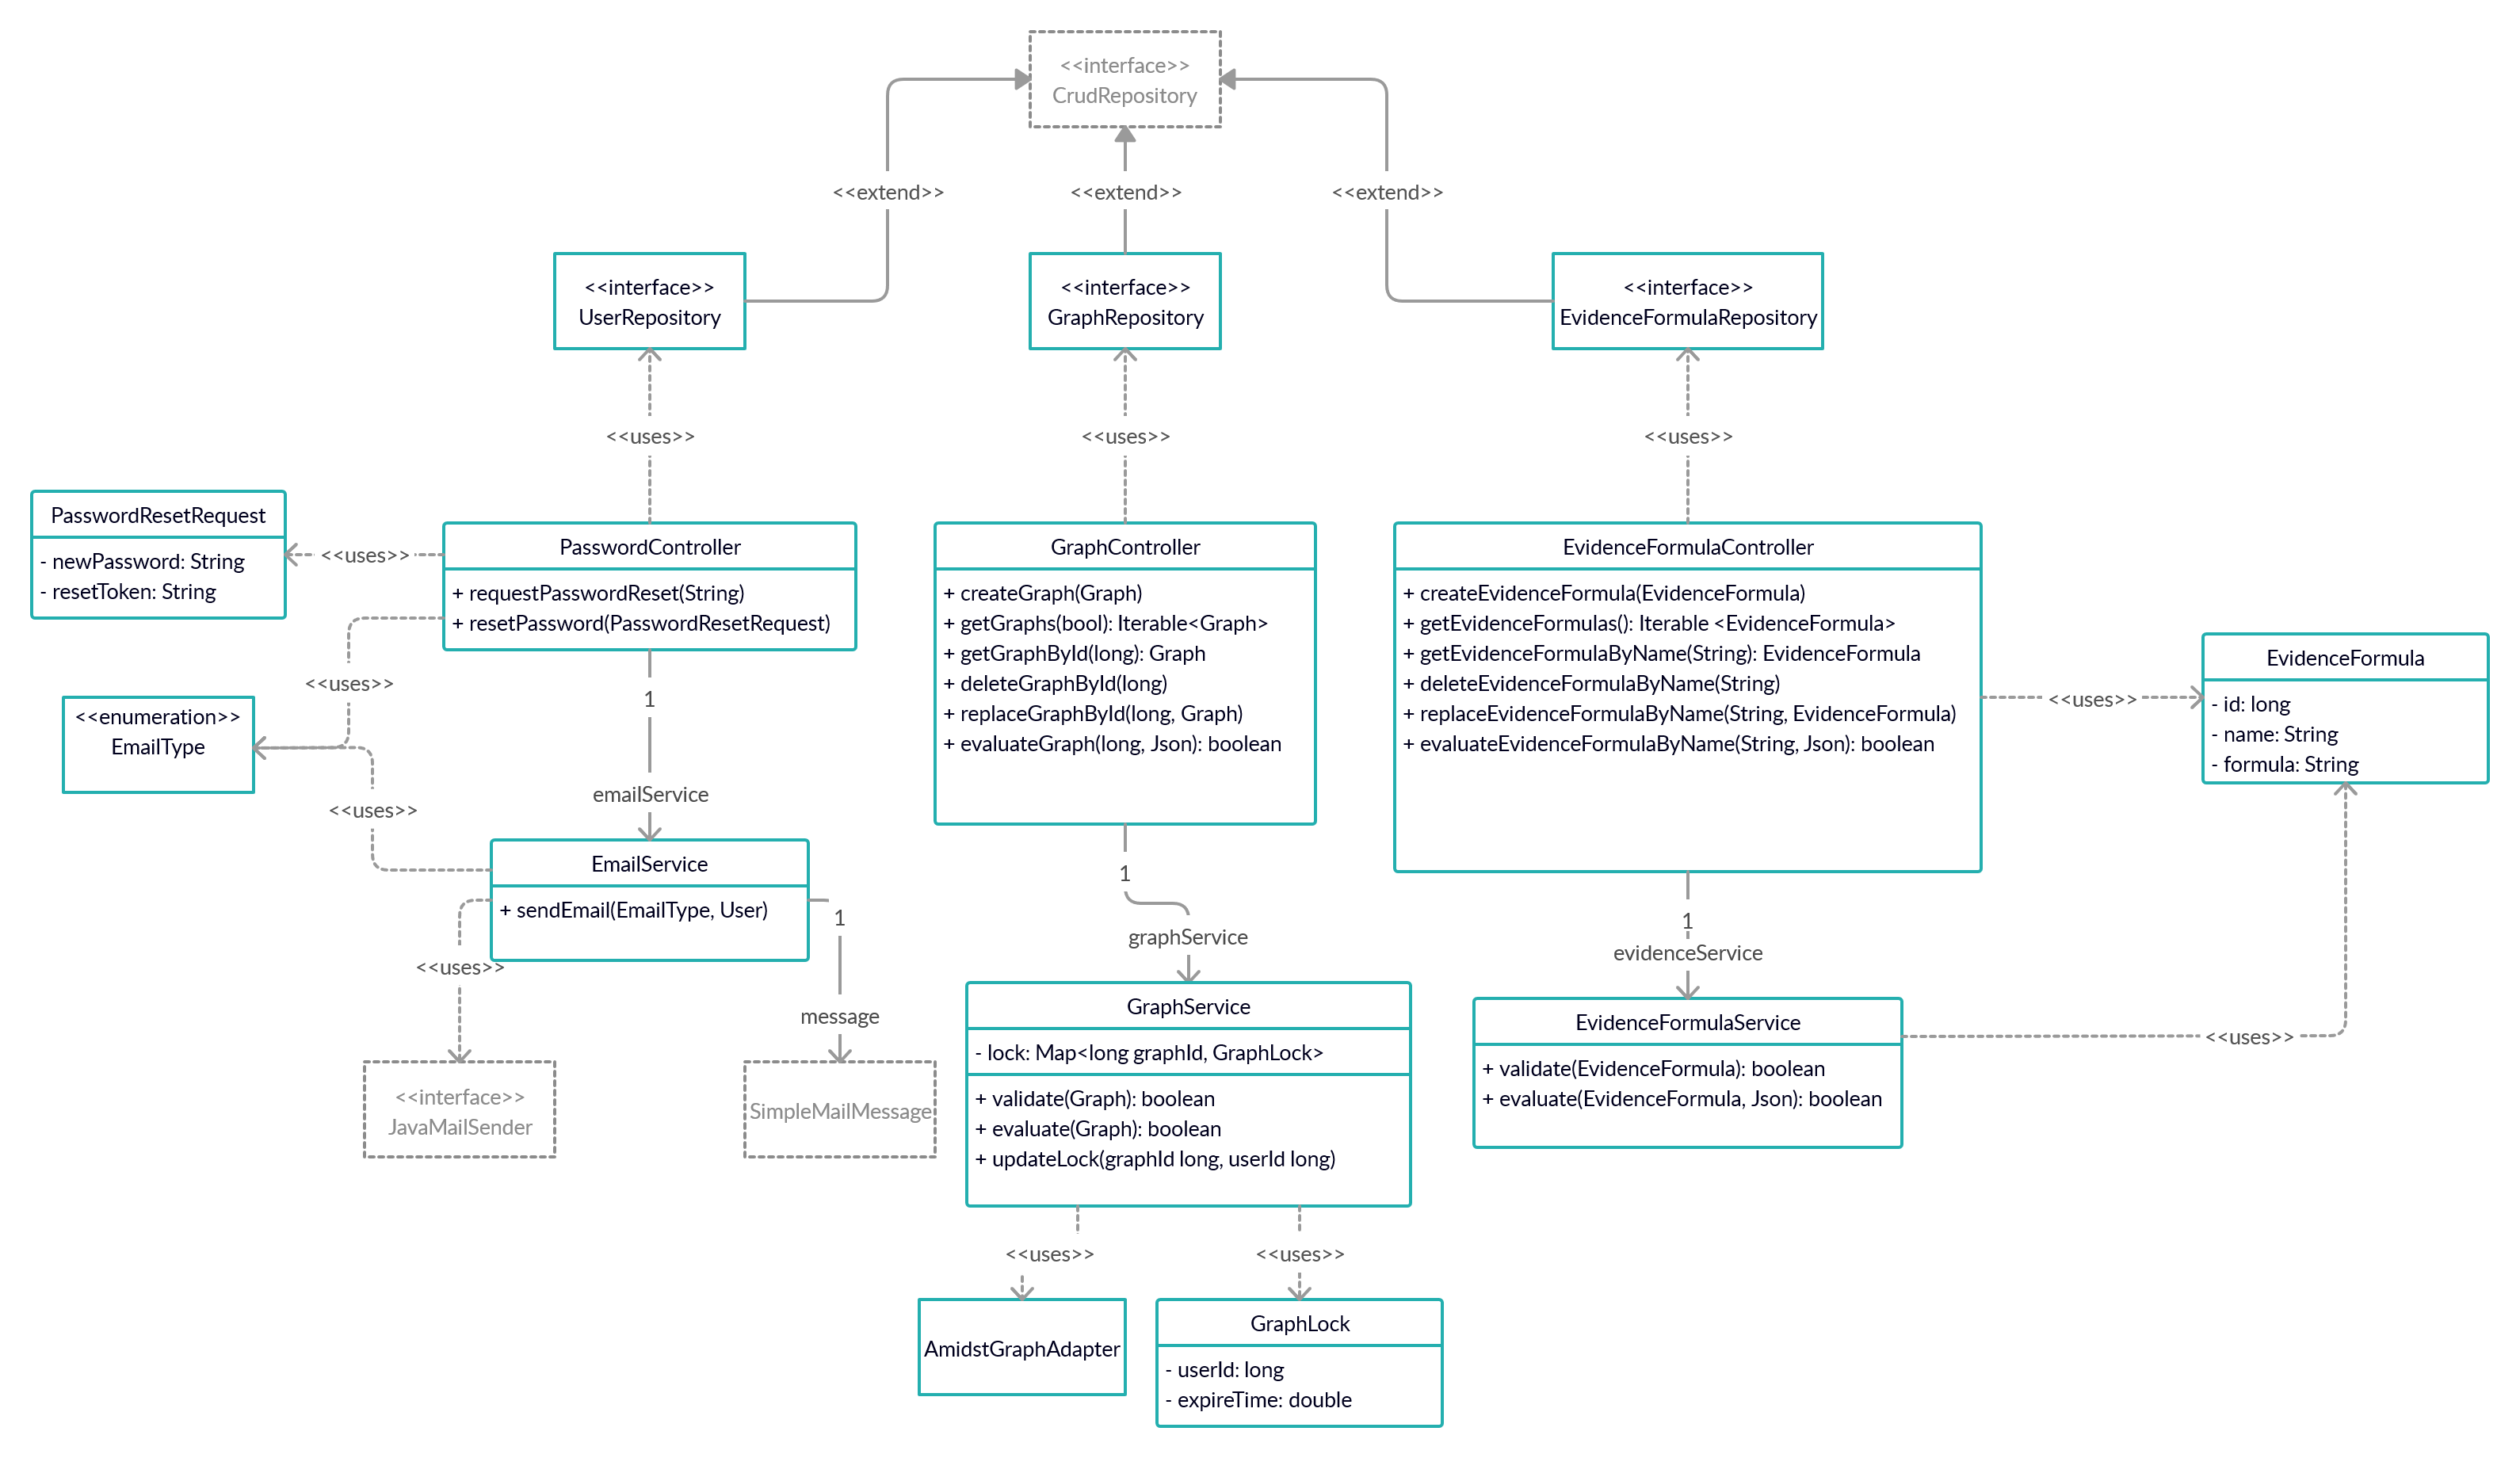
\includegraphics[width=\linewidth]{image/Rest_Controller.png}
    \caption{Klassendiagramm für REST Controller}
\end{figure}
\newpage

\subsection{Benutzer}
\begin{figure}[ht!]
    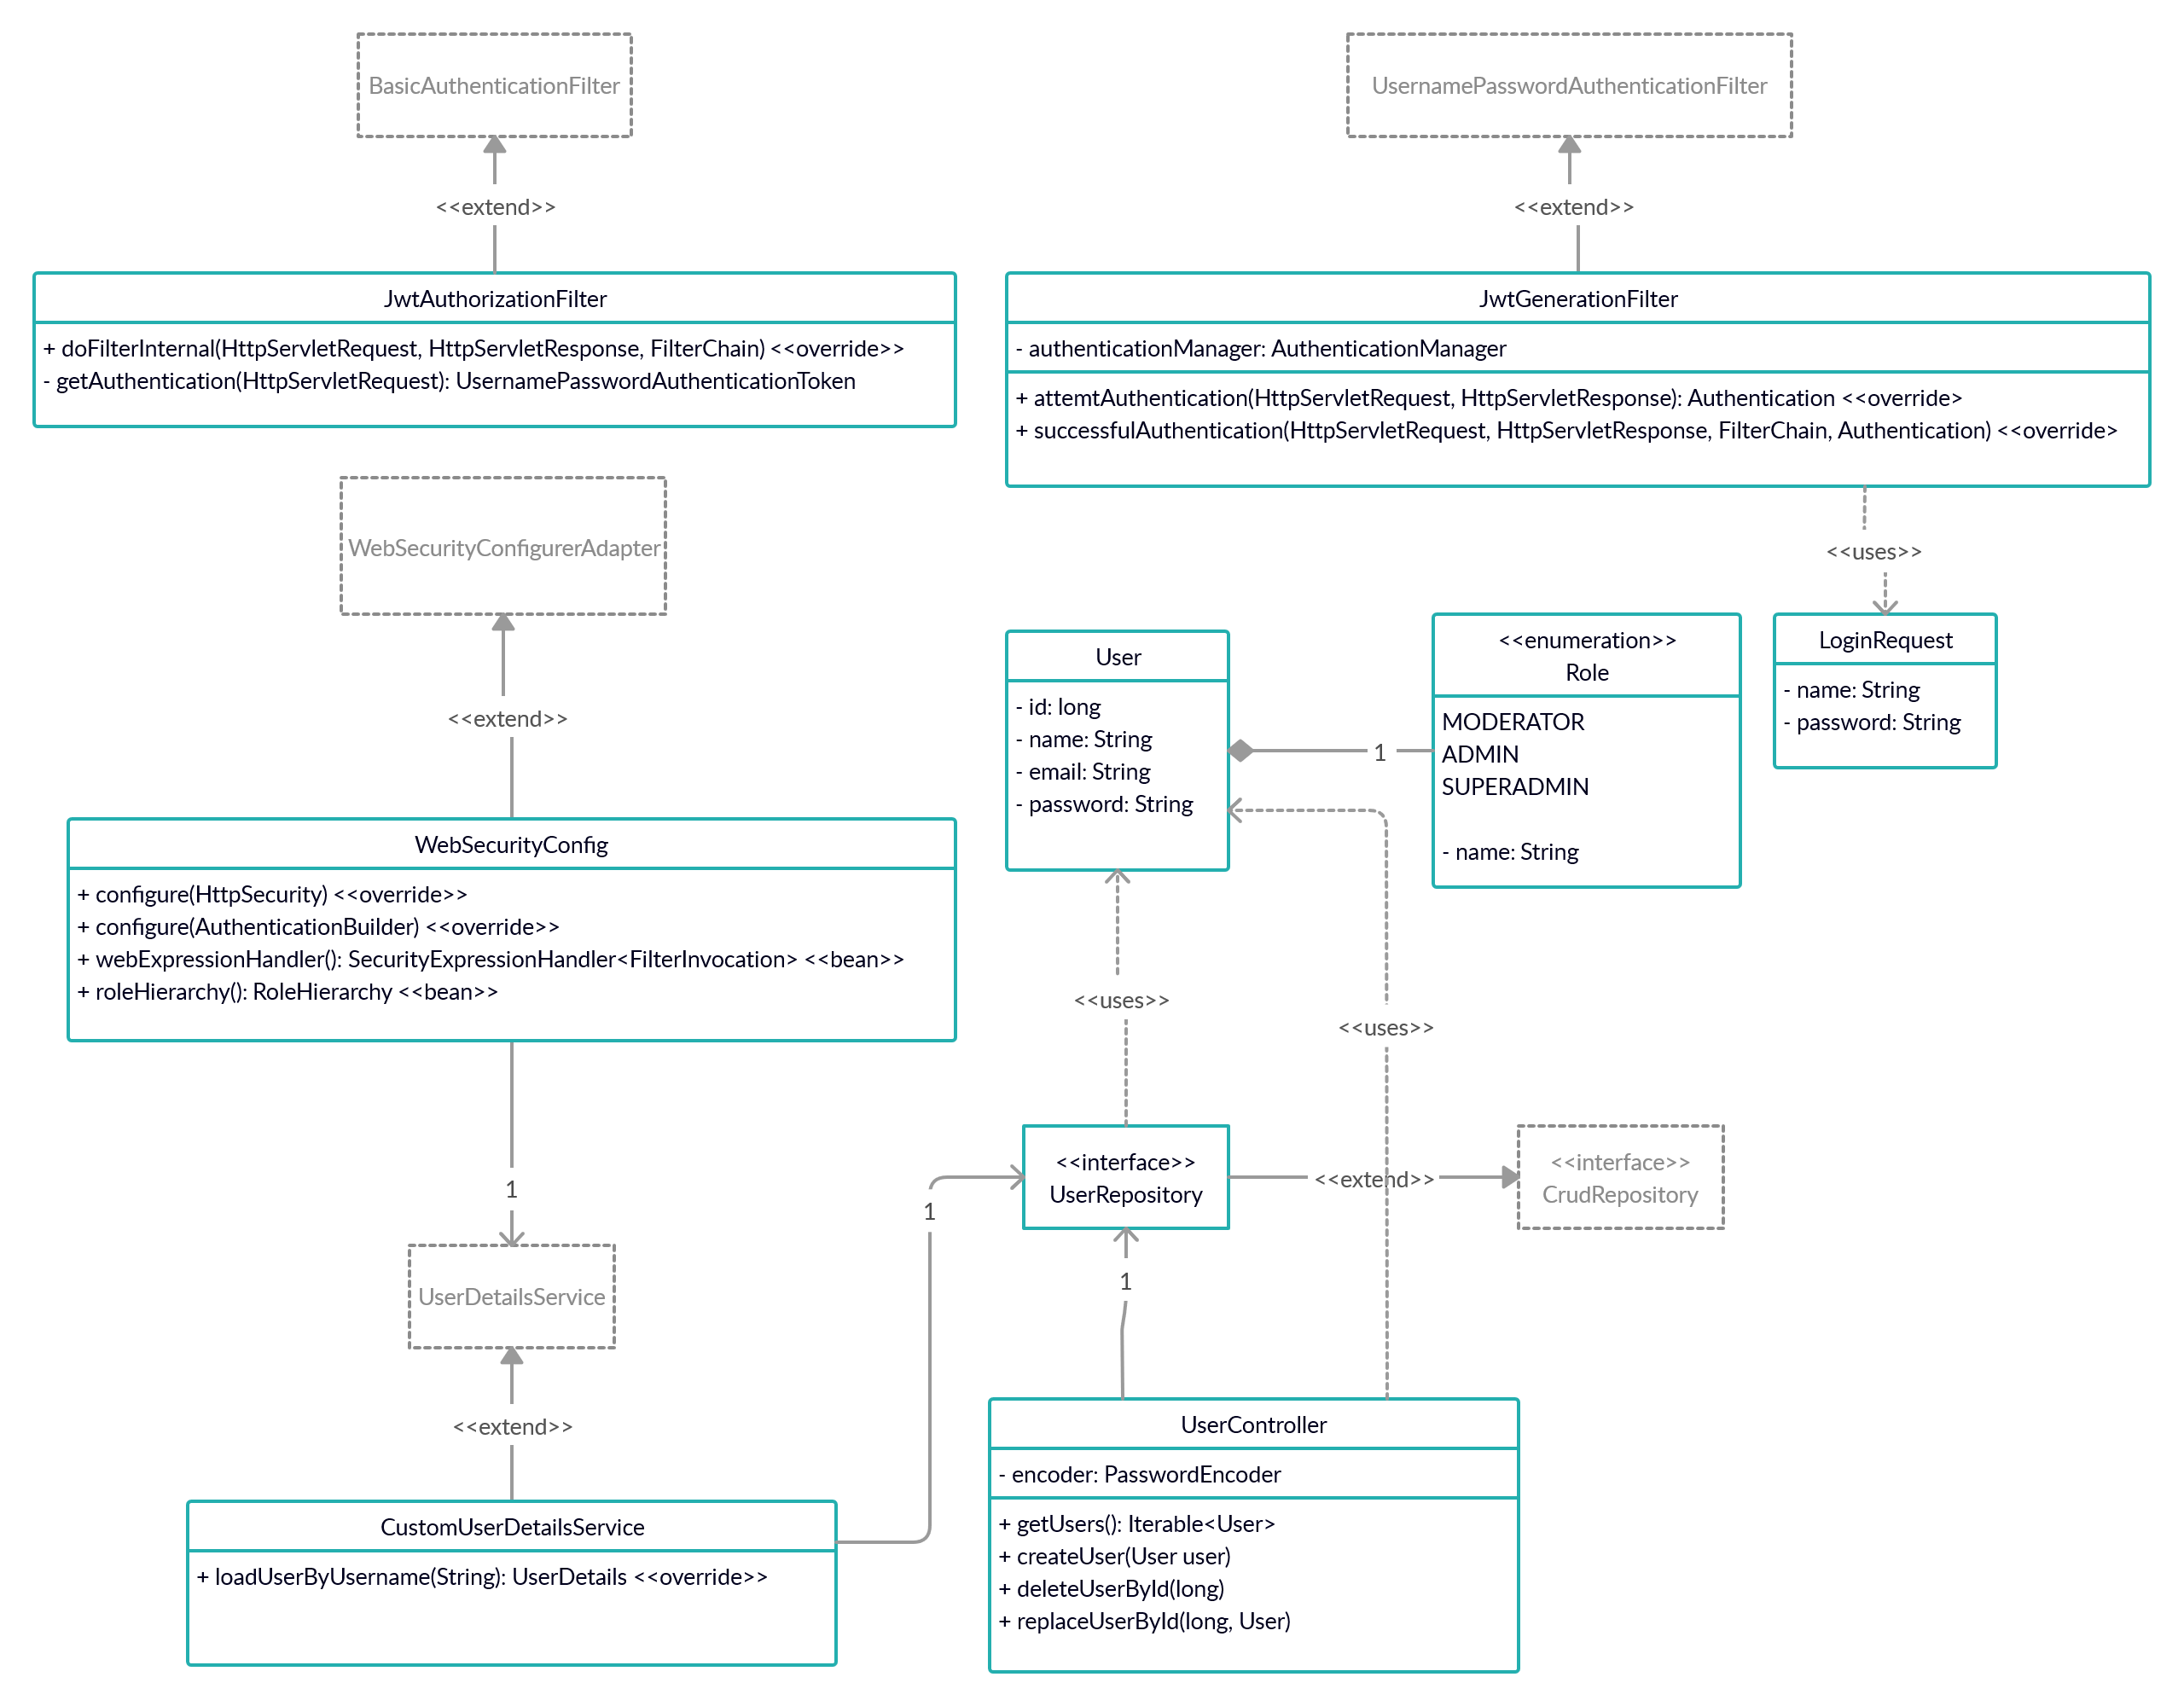
\includegraphics[width=\textwidth,height=\textheight,keepaspectratio]{image/LoginUser.png}
    \caption{Dieses Klassendiagramm beschreibt wie Benutzer im Backend definiert sind und wie sich ein Benutzer anmeldet. }
\end{figure}
\newpage

\subsection{Core}
\begin{figure}[ht!]
    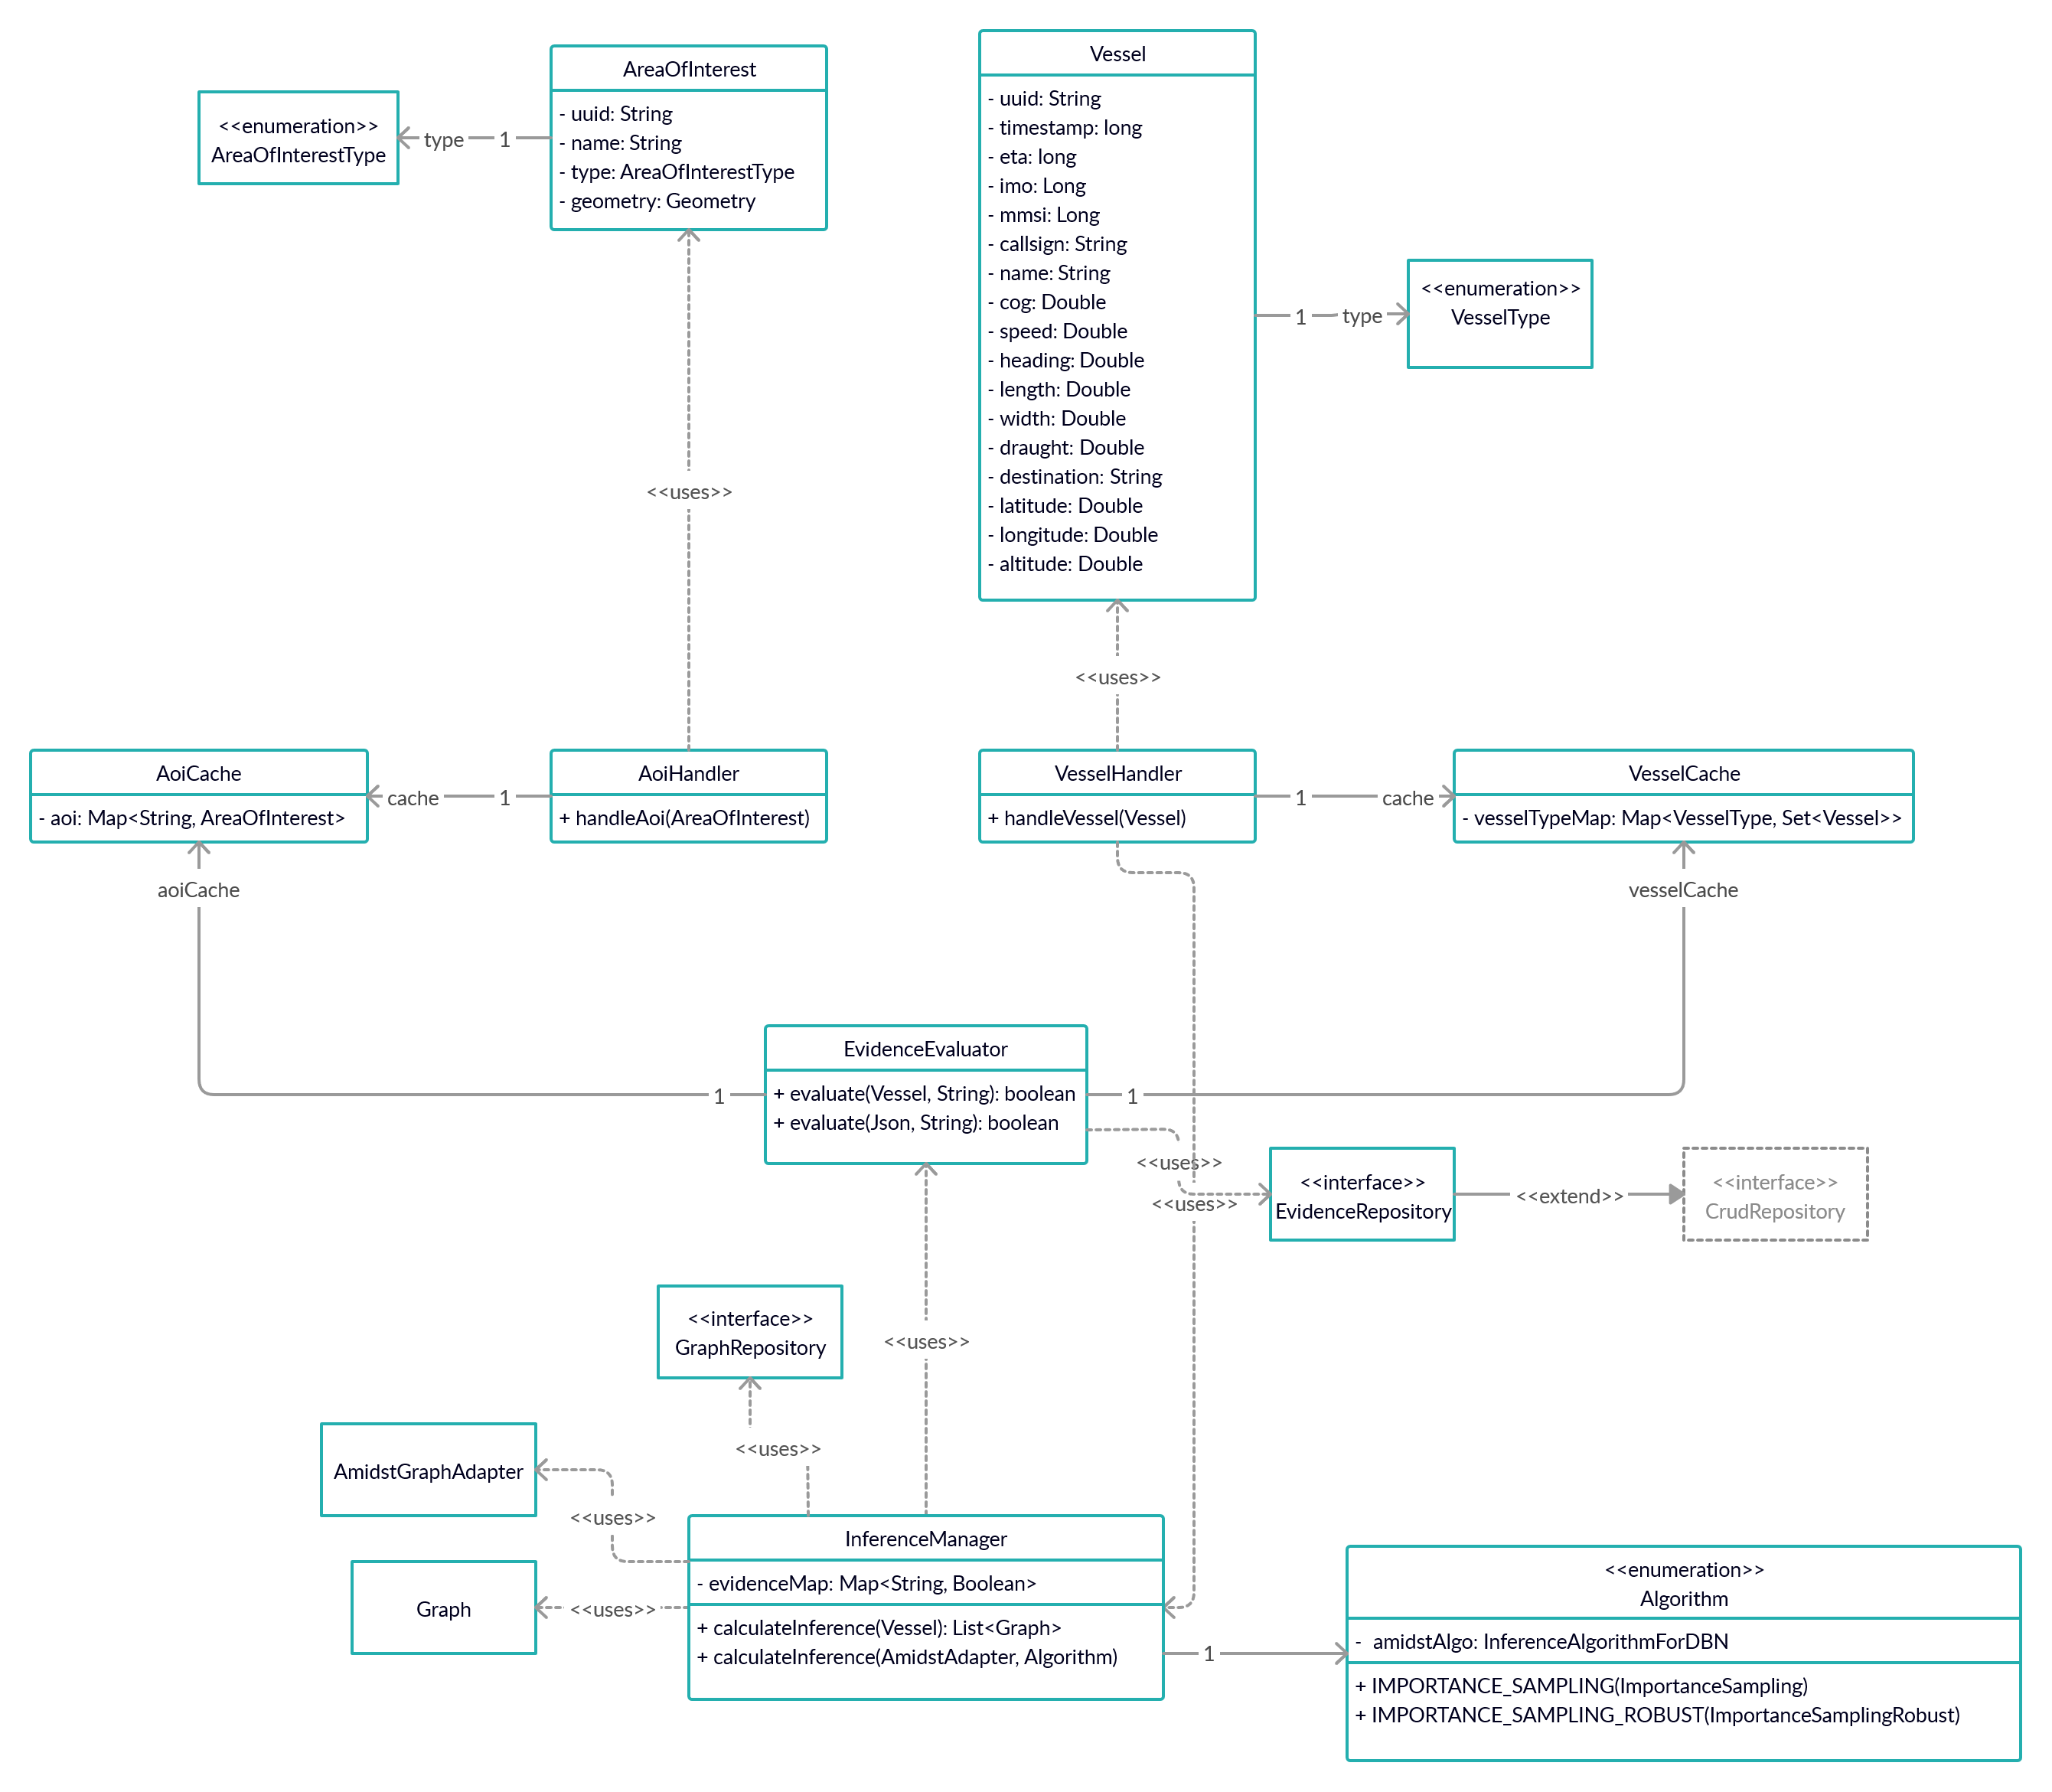
\includegraphics[width=\textwidth,height=\textheight,keepaspectratio]{image/Core.png}
    \caption{Dieses Klassendiagramm beschreibt die Kommunikation zwischen IOSB-Servern und der Inferenz-Engine.}
\end{figure}

\newpage
\subsection{Netze}
\begin{figure}[ht!]
    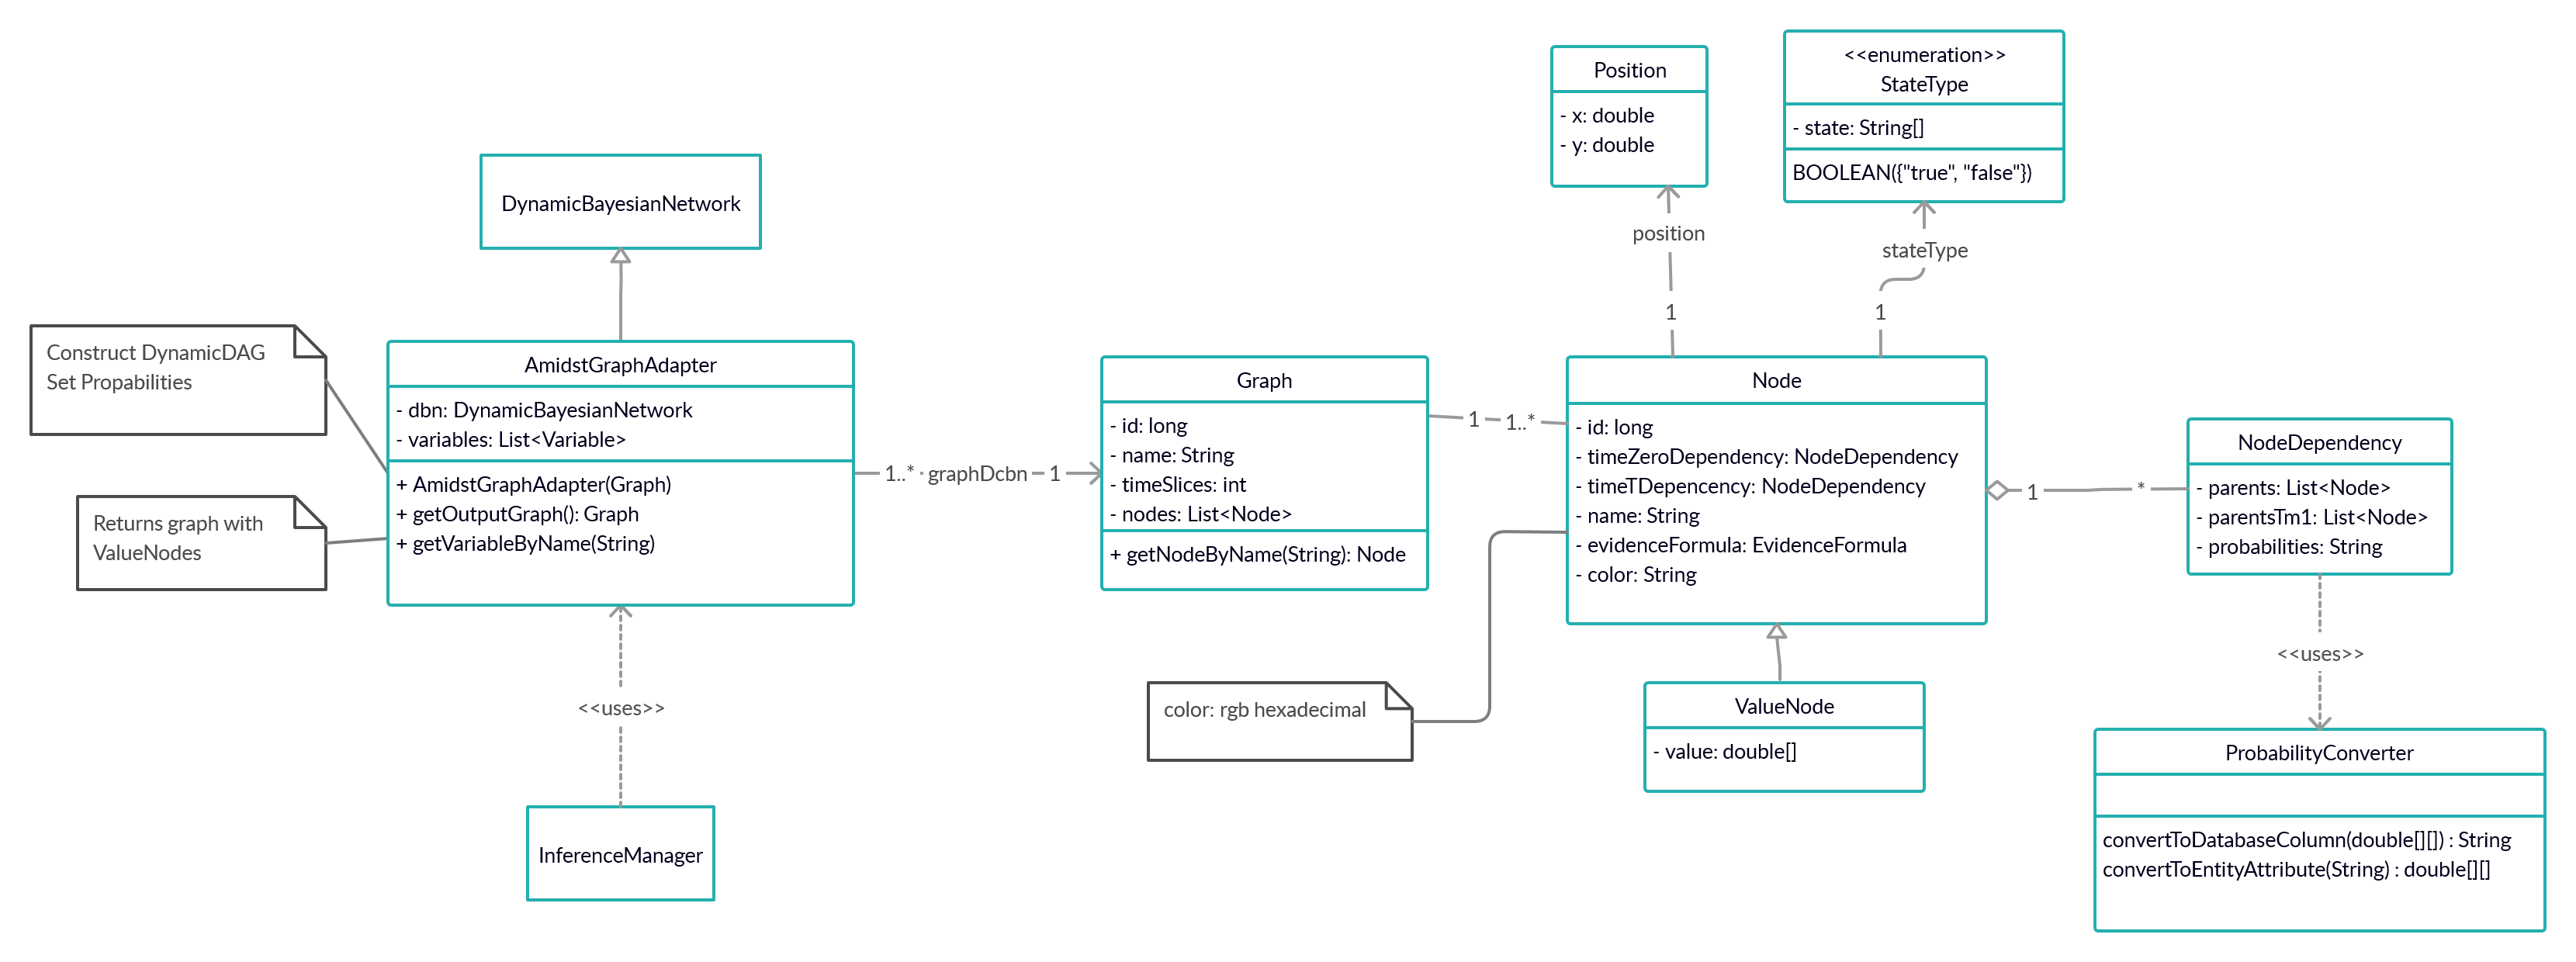
\includegraphics[width=\textwidth,height=\textheight,keepaspectratio]{image/Network.png}
    \caption{Dieses Klassendiagramm beschreibt wie Dynamische Bayes'sche Netze im Backend definiert sind. }
\end{figure}

\section{Sequenzdiagramme}

\subsection{Evaluierung eines Graphen}
\begin{figure}[ht!]
    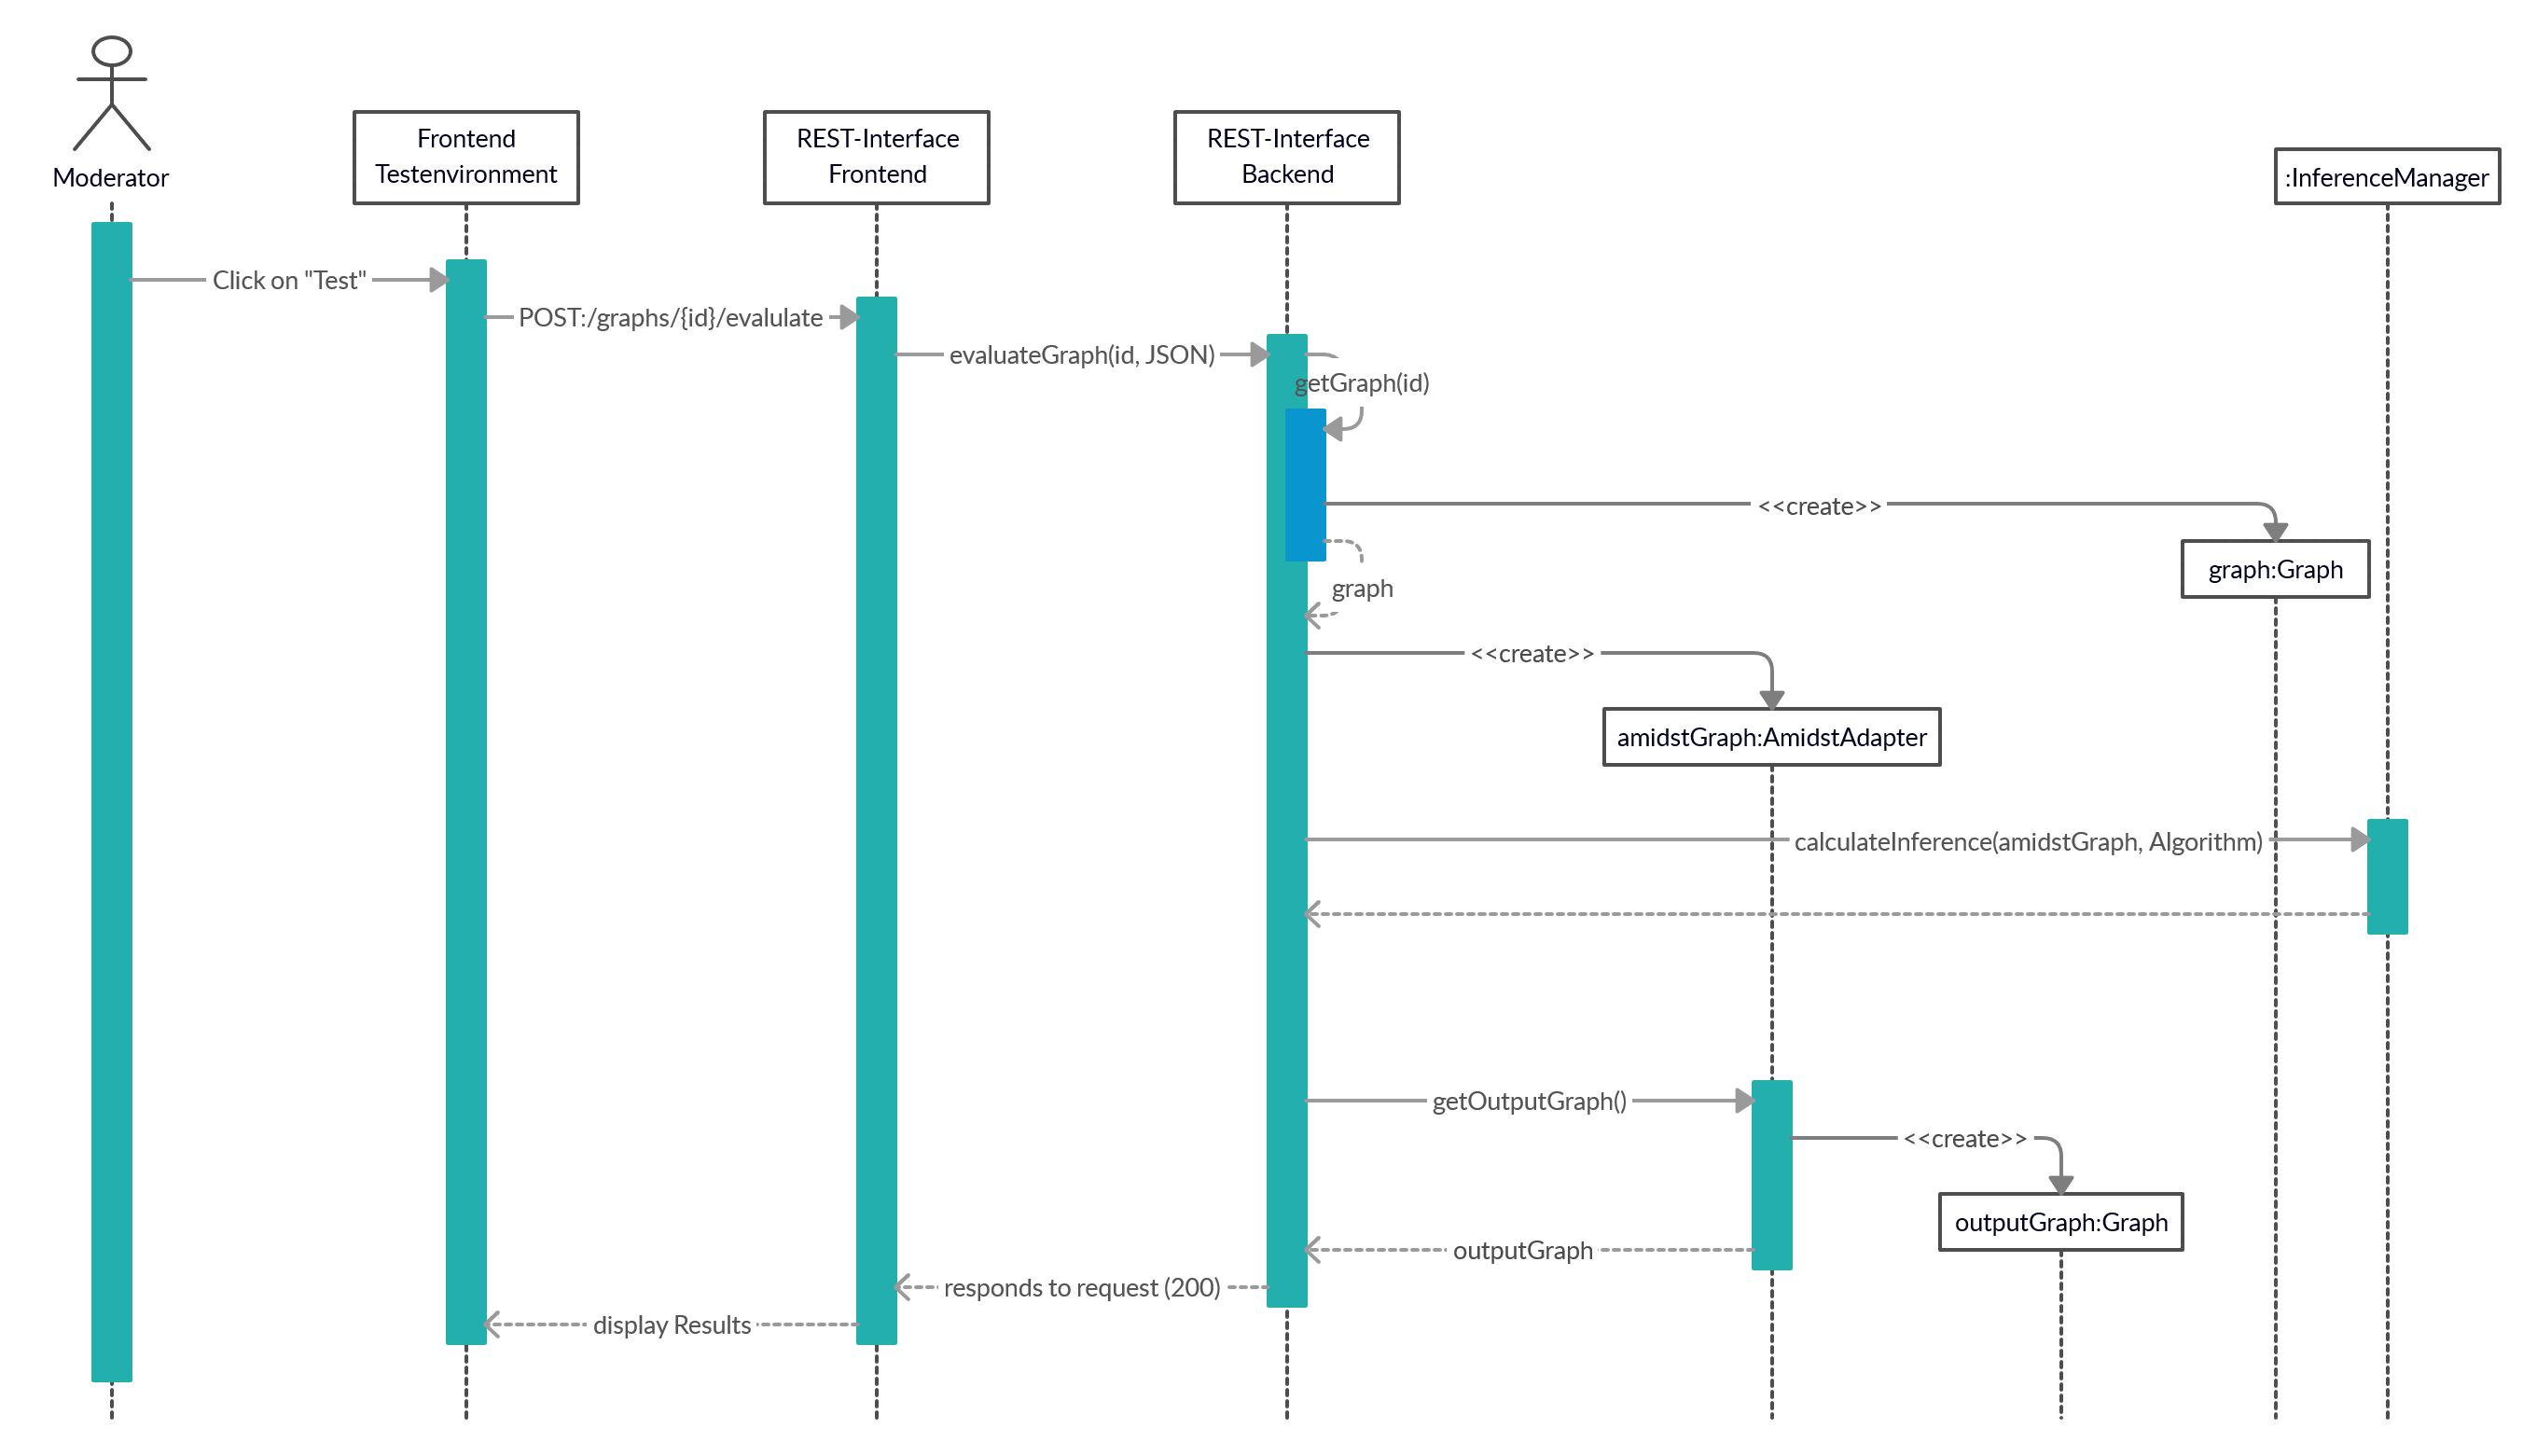
\includegraphics[width=\textwidth,height=\textheight,keepaspectratio]{image/SequenceEvaluateGraph.png}
    \caption{Dieses Sequenzdiagramm beschreibt wie die Inferenzen eines Graphens evaluiert werden.}
\end{figure}
\end{document}